\chapter{Completaci\'on de m\'odulos} \justifying
Sea $X$ un conjunto
\begin{defi}
Una \textbf{pseudom\'etrica} es una aplicaci\'on
$$\bt  d: X \times X \rar & \bb R^+ \\[-5mm] (x,y) \rarmaps & d(x,y) \et$$
con la propiedades sim\'etrica, reflexiva y triangular
$$d(x,y) = d(y,x) \qquad d(x,x)=0 \qquad d(x,y) \le d(x,z) + d(z,y)$$
que definen bolas 
$$B_{\varepsilon}(x) = \{y\in X \, /\, d(x,y) < \varepsilon\} \quad \varepsilon > 0$$ que a su vez definen la \textbf{topolog\'ia de las bolas}, cuyos abiertos son uni\'on de bolas. Construimos as\'i el espacio topol\'ogico $(X,\mc U_d)$ asociado a la pseudom\'etrica $(X,d)$. 
\end{defi}
\begin{obs}
    Para que una psudeom\'etrica sea m\'etrica hace falta que 
    $$d(x,y) = 0 \iff x=y$$
\end{obs}
\begin{prop}
    $(X,d)$ es m\'etrico $\iff (X,\mc U_d)$ es separado ($= T_2$). 
\end{prop}
\begin{dem}
    $\Rightarrow)$ Definiendo $\bar d = d(x,y)$ y las bolas $B_{\nicefrac{1}{3} \bar d} (x)$, $B_{\nicefrac{1}{3}\bar d} (y)$, no existe $z$ en ambas bolas pues contradir\'ia la desigualdad triangular.

    $\Leftarrow)$ Para cada $y\in X$ podemos encontrar $B_{\varepsilon}(x) \ni y$. 
\end{dem}
Sea $(X,d)$ un espacio pseudom\'etrico y $\big\{\{x_n\}_{n\in \bb N}\big\}$ el conjunto de las sucesiones en $X$, y consideramos $\mc C \subset Suc(X)$ las sucesiones de Cauchy, es decir, que verifican que
\begin{defi}
    $\{x_n\}$ es una \textbf{sucesi\'on de Cauchy} si para cada $\varepsilon \in\bb R^+$ existe $n_o \in \bb N$ tal que $$d(x_n,x_m)< \varepsilon \qquad \forall \, n,m \ge n_o$$ 
    Intuitivamente decimos que estas sucesiones convergen.
\end{defi}
\begin{defi}
    Dos \textbf{sucesiones de Cauchy} $\{x_n\} \sim \{y_n\}$ se dicen \textbf{equivalentes}, y se denota por $\{x_n\} \sim \{y_n\}$, si $\{d(x_n,y_n)\}$ es una sucesi\'on de Cauchy convergente a 0.
\end{defi}
\begin{defi}
    La \textbf{completaci\'on} de $(X,d)$ es el conjunto 
    $$\widehat X = \modulo{\text{Sucesiones de Cauchy}}{\sim}$$
\end{defi}
\begin{ejem}
    $\widehat {\bb Q} = \bb R$
\end{ejem}
\begin{prop}
    $(X,d) \longrightarrow (\widehat X, \widehat d)$ define una isometr\'ia de forma que $(\widehat X, \widehat d)$ es un espacio m\'etrico. Se define
    $$\bt  X \rar{\varphi} & \widehat X \\[-5mm] x \rarmaps & \{x\}_{n\in \bb N} \et$$
    y la distancia $\widehat d$ es 
    $$\widehat d\big([\{x_n\}],[\{y_n\}]\big) = \lim_{n\to \infty} d(x_n,y_n)$$
    de forma que hay que comprobar que si $[\{x_n\}], [\{y_n\}]$ son sucesiones de Cauchy, $d(x_n,y_n)$ es una sucesi\'on de Cauchy convergente, que existe ese l\'imite y no depende de los representantes, y adem\'as que verifica las propiedades de distacia. 

    El nuevo espacio m\'etrico $(\widehat X, \widehat d)$ es completo, toda sucesi\'on de Cauchy converge. 

    La isometr\'ia es inyectiva ($(X,d) \hookrightarrow (\widehat X, \widehat d)$) si y solo si $d$ es m\'etrica. 

    $(\widehat X, \widehat d)$ ya es m\'etrico pues $d(x,y) = 0 \iff \{x\} \sim \{y\}$.
\end{prop}
\begin{cor}
    Concluimos as\'i que todo espacio psuedom\'etrico se sumerge en un espacio m\'etrico completo, y es el m\'inimo, es decir, si $(X,d) \hookrightarrow (\widehat Y, \bar d)$ (con $\widehat Y$ otro espacio completo), entonces factoriza
    $$\bt (X,d) \rar[hook] \arrow{d} & (\widehat X, \widehat d) \arrow{dl} \\[5mm] (\widehat Y, \bar d) \et$$
    Es decir, $$Hom_{unif}((X,d), \widehat Y) = Hom_{unif} (\widehat X_d, \widehat Y)$$
\end{cor}
\begin{prop}
    Sea $(E,+)$ un grupo abeliano, consideremos pseudom\'etricas $d$ tales que $d(e+\bar e, e'+\bar e) = d(e,e')$. De forma que dar $d(0,e)=\|e\|$ es dar todas las distancias $d(e,\bar e) = d(0,e-\bar e)$. Se tiene tambi\'en la propiedad triangular, sim\'etrica y reflexiva 
    $$\|e+e'\|\le \|e\|+\|e'\| \qquad \|\lambda e\| = |\lambda| \|e\| \qquad \|e-e'\| = \|e'-e\|$$
\end{prop}
\begin{obs}
    Dadas dos distancias $d,d'$ si para cada $\varepsilon \in \bb R^+$ existe $\delta\in \bb R^+$ con 
    $$d(x,y) <  \delta \Rightarrow d'(x,y) < \varepsilon \quad  \equiv \quad B_{\delta}^d(x) \subset B_{\varepsilon}^{d'}(x) $$
    (que $d$ es m\'as fina que $d'$) y si se cumple tambi\'en que 
    $$d'(x,y) <  \delta' \Rightarrow d(x,y) < \varepsilon' \quad  \equiv \quad  B_{\delta'}^{d'}(x) \subset B_{\varepsilon'}^d(x)$$
    estas distancias definen la misma topolog\'ia, y ambas definen las mismas sucesiones de Cacuhy. 
\end{obs}
\section{Filtraciones}
Sea $M$ un $A$-m\'odulo, 
\begin{defi}
    Una \textbf{filtraci\'on en} $M$ es una cadena 
    $$M =M_o \supset M_1\supset M_2 \supset \cdots\supset M_n \supset \cdots \supset 0$$
\end{defi}
\begin{defi}
    Se define la \textbf{distancia} entre dos elementos de la \textbf{filtraci\'on}
    $$d(m,m') = \begin{cases}
        \dfrac{1}{2^i} & \text{ si } m-m'\in M_i - M_{i+1} \\[3mm] 0 & \text{ si } m-m'\in\displaystyle \bigcap_i M_i 
    \end{cases}$$
\end{defi}
\begin{prop} \,
    \begin{enumerate}[1)]
        \item $d$ es pseudom\'etrica en $M$.  
        \item $d$ es m\'etrica $\iff$ $\displaystyle \bigcap_{i\in \bb N} M_i = 0$
    \end{enumerate}
\end{prop}
\begin{defi}
    Se tiene as\'i en $M$ una topolog\'ia y se define $\widehat M$ el \textbf{completado de} $M$ por $\{M_i\}_{i \in \bb N}$. 
\end{defi}
\begin{prop}
    Dos filtraciones $\{M_i\}_{i \in \bb N}$, $\{M'_i\}_{i \in \bb N}$ definen m\'etricas equivalentes $\iff$ para cada $n \in \bb N $, existe $n_o$ tal que
    $$M_{n_o} \subset M_n'$$
    y rec\'iprocamente, para cada $n \in \bb N$ existe $n_o \in \bb N$ tal que 
    $$M_{n_o}' \subset M_n$$
\end{prop}
\begin{dem}
    Al lector.
\end{dem}
Sea $I$ un conjunto parcialmente ordenado de \'indices filtrante decreciente.
\begin{defi}
    Un \textbf{sistema proyectivo} es una familia de m\'odulos $\{\bar M_i\}_{i \in I}$ y para cada $i \le j$,  $\varphi_{ij} : \bar M_i \longrightarrow \bar M_j$ verficando que para cada $i \le j \le k$
    $$\bt \bar M_i \rar{\varphi_{ij}} \arrow[bend right=10mm]{rr}{\varphi_{ik}}& \bar M_j \rar{\varphi_{jk}} \rar & \bar M_k \et \qquad \boxed{\varphi_{ik} = \varphi_{jk} \circ \varphi_{ij}}$$
    \end{defi}
\begin{ejem}
     Podemos usar los naturales como \'indices $I = \bb N$, pero invertimos el orden para que sea filtrante decreciente, para cada $i,j \in I$ existe otro $k \le i,j$ con
     $$\bt \cdots \rar{\varphi_{43}} & M_3 \rar{\varphi_{32}} & M_2 \rar{\varphi_{21}} & M_1\et$$
\end{ejem}
\begin{defi} Se define el \textbf{l\'imite proyectivo} del sistema proyectivo como
    $$\varprojlim M_i = \left\{(m_i)_{i \in I} \in \prod M_i \, / \, \varphi_{ij}(m_i) = m_j \text{ si } i \le j \right\} $$
\end{defi}
\begin{obs}
    Si $I=\bb N$, intuitivamente
    $$\bt \varprojlim M_i \rar 
    &\cdots \rar{\varphi_{43}} & M_3 \rar{\varphi_{32}} & M_2 \rar{\varphi_{21}} & M_1\et$$
\end{obs}
\begin{prop}
    $\varprojlim M_i \subset \prod M_i$ es un subm\'odulo, que induce
    $$\bt \varprojlim M_i \subset \rar[hook] \arrow{dr}{\varphi_i} & \prod M_i \arrow{d}{\pi_i} \\[5mm] & M_i \et$$
    y se tienen los tri\'angulos conmutativos
    $$\bt \varprojlim M_i \subset \rar{\varphi_i} \arrow{dr}{\varphi_j} & \prod M_i \arrow{d}{\varphi_{ij}} \\[5mm] & M_j \et \qquad \text{ si }i \le j$$
\end{prop}
\begin{propi}
    [Universal] Se tiene que 
    $$Hom_A(N,\varprojlim M_i) = \varprojlim Hom_A(M,M_i)$$
    que nos dice que
    $$N \longrightarrow \varprojlim M_i \text{ es morfismo } \iff  \bt N \rar{T_i} \arrow[swap]{dr}{T_j} & M_i \arrow{d}{\varphi_{ij}} \\ & M_j \et \text{ es conmutativo.}$$
\end{propi}

Dada una filtraci\'on $M  = M_o \supset M_1 \supset \cdots \supset M_n \supset \cdots $ consideramos los cocientes
$$\cdots \longrightarrow \modulo{M}{M_2} \longrightarrow \modulo{M}{M_1} \longrightarrow \modulo{M}{M_o} = 0$$
siendo los morfismos las proyecciones naturales, que es un sistema proyectivo, y tiene por l\'imite proyectivo $\varprojlim \modulo{M}{M_i}$ y $M$ factoriza por \'el, no es igual a $M$ ni tampoco a $\modulo{M}{\bigcap M_i}$, es algo m\'as rico.

Se tienen los morfismos 
$$\bt \modulo{M}{M_j} \rar{\pi_{ij} } & \modulo{M}{M_i} \et \quad M_i \supset M_j  \text{ si } i \le j$$
y $[n_i]_i \in \modulo{M}{M_i}$, con $\pi_{ij}(m_j) = m_i \mod M_i$, $[m_{j}]_i = [m_i]_i$, por lo que se tiene el sistema proyectivo $(n_i)$ con $n_i - n_j \in M_i$ si $i\le j$.
\begin{teo}
    $\widehat M = \varprojlim \modulo{M}{M_i}$.
\end{teo}
\begin{lem}
    Sea $\{x_i\}_{i \in \bb N} \subset X$ una sucesi\'on de Cauchy, cualquier subsucesi\'on $\{x_{n_i}\}_{i \in \bb N} \subset \{x_n\}_{i \in \bb N}$ es de Cauchy y equivalente a $\{x_i\}_{i \in \bb N}$
\end{lem}
\begin{dem}
    Usar la convergencia de ambas, y la distancia entre ellas. 
\end{dem}
\begin{defi}
    Una \textbf{serie en la filtraci\'on} de una familia de elementos $\{m_i\}_{i \in \bb N}$ con $m_i\in M_i$ es la suma formal $$\sum_{i=0}^{\infty} m_i = \left( \sum_{i=0}^{n-1} m_i \right)_{n \in \bb N}$$
    y son siempre de Cauchy, pues 
    $$\sum_{i=0}^{n-1} m_i-\sum_{i=0}^{m-1} m_i = \sum_{i=m}^{n-1} m_i \in M_m \Rightarrow 
    d\left(\sum_{i=0}^{n-1} m_i, \sum_{i=0}^{m-1} m_i\right) \le \frac{1}{2^m} \qquad m \le n$$
\end{defi}
\begin{lem}
    Consideremos $\{M_i\}_{i \in \bb N}$ una filtraci\'on de $M$, toda sucesi\'on de Cauchy es equivalente a una serie, es decir, $\displaystyle (n_i)_{i \in \bb N} \sim \left( \sum_{i=0}^{\infty} m_i \right)$
\end{lem}
\begin{dem}
    $(n_i)_{i \in \bb N} $ de forma que para cada $i$ existe $j_i \in \bb N$ tal que $d(n_s,n_k) \le \frac{1}{2^i}$ con $s,k \ge j_i$. Escogemos entonces la subsucesi\'on $(n_{j_i})_{i \in \bb N}$, que por el primer lema es equivalente a la original. Si renombramos $(n_{i_j})_{i \in \bb N} = (\bar n_i)_{i \in \bb N}$, entonces 
    $$d(\bar n_i, \bar n_j) = d(n_{j_i}, n_{j_j}) \le \frac{1}{2^i} \Rightarrow \bar n_i -\bar n_j \in M_i \quad i \le j$$
    es decir, es una subsucesi\'on de forma que cada t\'ermino dista del siguiente lo justo para estar en $M_i$. 

    Por la teor\'ia de operadores, $\Delta \left(\sum _{0}^{n-1} m_i \right) = m_n$, $\Delta(\bar n_i) = \bar n_{i+1} - \bar n_i = m_i \in M_i$ es una sucesi\'on tal que el t\'ermino $i$-\'esimo est\'a en $M_i$. De forma que 
    $$\sum_{i=0}^{n-1}m_i = \bar n_n$$
    por tener las dos la misma diferencial, es decir, $$\bar n_n = \frac{1}{\Delta} (\Delta \bar n_n) = \frac{1}{\Delta} (\bar m_n) = \sum_0^{n-1} \bar m_i$$
    y como si dos series tienen la misma diferencial difieren una constante
    $$n_i = \frac{1}{\Delta} (\Delta n_i) + n_o' = \frac{1}{\Delta}(m_i) + n_o' = \sum_{j=0}^{i-1} m_j  + n_o' = \sum_{j=0}^{i-1} m_j \qquad (\text{tal que } m_o = m_o + n_o')$$ 
    damos valor cuando $n=1$, $\bar m_o = (\Delta \bar n_m )_o = \bar n_1 - \bar n_o$ y redefinimos la serie como $n_o+ \sum_{0}^{\infty} \bar m_o$.  

    Y toda sucesi\'on de Cauchy es equivalente a una serie, $\sum_0^{n-1} m_i = \bar n_n$
\end{dem}
\begin{dem}[del Teorema]
    Se tiene $M \longrightarrow \modulo{M}{M_i}$, veamos qu\'e hacemos corresponder a qu\'e. Recordemos que $\widehat M = \{[(n_i)_{i \in \bb N}] \text{ de Cauchy}, n_i \in M\}$ y 
    $$\varprojlim \modulo{M}{M_i} = \{([\bar n_i])_{i \in \bb N} \, / \, \bar n_i - \bar n_j \in M_j \text{ si } i \ge j \}$$ 
    $$\bt \widehat M \rar & \varprojlim \modulo{M}{M_i}  \\[-5mm] (n_i)_{i\in I} = (\sum^{i-1} m_j) \rarmaps & \left(\left[\sum_{j=0}^{i-1} m_j \right]_i\right) \et$$
    y 
    $$\bt \modulo{M}{M_i} \rar & \modulo{M}{M_{i-1}} \\[-5mm] [\sum^{i-1} m_j ]\rarmaps & [\sum^{i-2}m_i] = [\sum^{i-1} - m_{i-1}] \et$$
    y del rev\'es, $(n_i)$ va a parar a $n_i = n_{i-1} \mod M_{i-1}$, de forma que $([n_i])$ es de Cacuhy, y 
    $$\bt \widehat M \rar & \varprojlim \modulo{M}{M_i}  \\[-5mm] (n_i) & \arrow[mapsto]{l} ([n_i]) \et$$ 
\end{dem}

Dado un $A$-m\'odulo $M$ y una filtraci\'on $M = M_o \supset M_1 \supset \cdots \supset M_i \supset \cdots$, que define una pseudom\'etrica con una distancia $d(m,m') \le \frac{1}{2^i}, \, m-m'\in M_i$, y se pueden hablar de las sucesiones de Cacuhy, y que son equivalentes cuando la distancia entre los t\'erminos de las dos sucesiones tiende a 0, definiendo as\'i el completado de $M$, $\widehat M$. De forma que si $\{n_i\}$ es de Cauchy, $\{n_i'\}$ otra, $n_i' - n_{i+1} \in M_i$, lo que permite demostrar la igualdad
$$\bt \widehat M \rar[equal] & \varprojlim \modulo{M}{M_i} \\[-5mm] (n_i)_{i \in I} \rarmaps & (\bar n_i)_{i \in \bb N} \\[-5mm](n_i)_{i \in I} & \arrow[mapsto]{l} (\bar n_i) \et$$
siendo $\bar n_i$ la clase de $n_i \mod M_i$. Y del rev\'es, tal que la familia $(n_i)$ cumplan que $n_i-n_{i+1} \in M_i$.

Adem\'as, toda sucesi\'on de Cauchy es equivalente a una serie $\sum_i m_i$ con $m_i \in M_i$. De forma que el elemento $i$ es $\left( \left[\sum_j^{i-1} m_i \right]\right)_{i \in \bb N} $. De forma que se denota $(n_i)_{i \in \bb N} \sim \sum_{i=0}^{\infty} m_i$ y cada $n_i = n_{i-1} + m_{i-1} = n_{i-2} + m_{i-2} + m_{i-1} = \cdots  = \underbrace{n_o=m_o}_{\in M_o}+ m_1 + m_2 + \cdots + m_{i-1} $, que ahora ya es m\'etrica y se tiene el morfismo de completaci\'on 
$$\bt M \rar{\varphi} & \widehat M \\[-5mm] m \rarmaps & (m)_{i \in \bb N} \et \qquad \ker \varphi = \bigcap_{i \in I} M_i$$
\begin{ejem}
    Sea $A$ con $\alpha \subset A$ un ideal, $M$ un $A$-m\'odulo, escogemos la filtraci\'on $M_i = \alpha^n \cdot M $, es $$M_o = M \supset \alpha M \supset \alpha^2 M \supset \cdots \supset \alpha^n M \supset \cdots $$
\end{ejem}
\section{Exactitud de la completcai\'on}
Sea la sucesi\'on exacta de m\'odulos
$$\bt 0\rar & N \rar{i} & M \rar{\pi} & \bar M \rar & 0 \et$$
pudiendo identificar $N\subset M$ y $\bar M = \modulo{M}{N}$, y la filtraci\'on en $M$: $M  = M_o \supset M_1 \supset \cdots \supset M_n \supset \cdots$, tenemos filtraciones en $N$: $\{N \cap M_i\}_{i\in \bb N}$ y en $\bar M$: $\{\pi(M_i)\}_{i\in \bb N}$

\begin{teo} La sucesi\'on
$$\bt 0\rar & \widehat N \rar{\widehat i} & \widehat M \rar{\widehat \pi} & \widehat {\bar M} \rar & 0 \et$$
es exacta.
\end{teo}
\begin{obs}
    La exactitud se conserva por mantener las topolog\'ias inducidas en $N$ y $\bar M$ como cociente. 
\end{obs}
\begin{dem}
    $$\bt 0\rar & N \rar & M \rar{\pi} \arrow{dr} \arrow[squiggly]{d} & \bar M \arrow{d} \rar & 0 \\[5mm] 0 \rar & \modulo{N}{N \cap M_i} \rar & \modulo{M}{M_i} \rar{ \pi_i} & \modulo{\bar M}{\pi(M_i)}  \rar[dashed] & 0  \et$$
    de forma que 
    $$\ker \pi_i = \pi^{-1}_i (\pi(M_i)) = \modulo{M_i + N }{M_i} \simeq \modulo{N}{N \cap M_i}$$ 
    por ser $\pi^{-1}(\pi(N)) = M'+\ker \pi$. 

    El problema queda en la epiyectividad. 

    Para completar $\widehat {\bar M}$ escogemos elementos suyos, que son de la forma $[\sum_i\pi(m_i)]$ y $\widehat \pi$ identifica $[\sum m_i] \mapsto [\sum_i\pi(m_i)]$, pero no siempre es epiyectivo. 
\end{dem}
\begin{ejem}
    Volviendo al ejemplo de la filtraci\'on $\alpha$-\'adica, $N \cap \alpha^nM \supset \alpha^n N$ y esto hace que sea exacta, pues las completaciones son equivalentes. 
\end{ejem}
\begin{ejem}
    [Topolog\'ia y completaci\'on $\alpha$-\'adica] Sea $A$ anillo y $\alpha \subset A$ ideal, para un $A$-m\'odulo $M$ su topolog\'ia $\alpha$-\'adica es $\{\alpha^i \cdot M\}_{i \in \bb N}$. En particular, $\widehat A$ es anillo (producto de sucesiones, comprobar), y se tiene el morfismo de anillos
    $$\bt A \rar & \widehat A \\[-5mm] a \rarmaps & \left[(a)_{i \in \bb N} \right] \et$$
     de forma que $\widehat M$ no solo es $A$-m\'odulo, es tambi\'en $\widehat A$-m\'odulo con el producto
     $$(a_i)\cdot (n_i) = (a_i \cdot n_i)_i$$
     que no depende del representante elegido. 
\end{ejem} 
\begin{defi}
    Se dice que una filtraci\'on $\{M_i\}_{i \in \bb N}$ en $M$ es una \textbf{$\alpha$-filtraci\'on} si $\alpha M_i \supset M_{i+1} \, \forall \, i$. Llamaremos \underline{la} $\alpha$-filtraci\'on a $M\supset \alpha M \supset \cdots \supset \alpha^i M \supset \cdots$, que tambi\'en llamaremos can\'onica. Se dice que una $\alpha$-filtraci\'on es \textbf{$\alpha$-estable} si $\alpha M_i = M_{i+1}$ con $i\ge n_o$. 
\end{defi}
\begin{lem}
    Las $\alpha$-filtraciones son equivalentes a \underline{la} $\alpha$-filtraci\'on. Si $\{M_i\}_{i \in \bb N}$ es $\alpha$-estable, entonces $\{M_i\}_{i \in \bb N}\sim \{\alpha^i M\}_{i \in \bb N}$. 
\end{lem}
\begin{dem}
    Por ser $\{M_i\}_{i \in \bb N}$ una $\alpha$-filtraci\'on, entonces, $\alpha^i M =\alpha^iM_o \subset M_i \forall \, i$. 

    Para la inclusi\'on contraria, cada $M_i \subset M_o =M$ a partir de cierto $i$. Consideramos $n_o \in I$ y como $\alpha M_i = M_{i+1}$, es decir, $M_{n_o+h} \subset \alpha^h M$, porque $M_{n_o} \subset M \Rightarrow M_{n_o+h} = \alpha^h M_{n_o} \subset \alpha^h M$.  
\end{dem}
\begin{defi}
    Sea $A$ anillo e $\alpha$ ideal de $A$, definimos el \textbf{dilatado de }$A$ \textbf{por} $\alpha$ como
    $$D_{\alpha} A = A \oplus \alpha \oplus \alpha^2 \oplus \cdots  \oplus \alpha^i \oplus \cdots = A[t\alpha] $$
    que es una $A$-\'algebra graduada. Y sus elementos son de la forma $ \displaystyle \sum_i t^i \alpha_i, \, \alpha_i \in \alpha^i =\bigoplus_i \alpha_i$ y con el producto usual de polinomios.
\end{defi}
\begin{prop}
    Si $\alpha$ es finito generado, $\alpha=(a_1, \ldots, a_n)$, entonces $$ \bt A[x_1, \ldots, x_n] \rar & D_{\alpha} A \arrow{rr} &[-13mm] & 0 \\[-5mm] x_1, \ldots, x_n \rarmaps & \alpha_1, \ldots, \alpha_n &[-13mm] \in 0 \oplus \alpha \oplus 0 \oplus \cdots   \et$$
\end{prop}
Sea $A$ anillo, $\alpha \subset A$ finito generado y $M$ un $A$-m\'odulo finito generado,
\begin{teo}
    Una $\alpha$-filtraci\'on $\{M_i\}_{i \in \bb N}$ de m\'odulos finito generados es estable si y solo si
    $$DM = M \oplus M_1 \oplus M_2 \oplus \cdots \oplus M_i \oplus \cdots $$
    es un $D_{\alpha}A$-m\'odulo finito generado. 
\end{teo}
\begin{dem}
    $\Rightarrow) \, \alpha M_i = M_{i+1}$ para cierto $i \ge n_o$ y $M_{n_o+h} = \alpha^h M_{n_o}$, $M_o\oplus M_1 \oplus \cdots \oplus M_{n_o}$ genera $\bigoplus_i M_i$ como $D_{\alpha}A$-m\'odulo (por ejemplo $\cdots \oplus 0\oplus M_{n_o+h} \oplus 0 \oplus \cdots= (\cdots \oplus 0\oplus \alpha_h \oplus 0 \oplus \cdots)(\cdots \oplus 0\oplus M_{n_o} \oplus 0 \oplus \cdots)$). Por tanto, $M_o\oplus M_1 \oplus \cdots \oplus M_{n_o}$ es un $A$-m\'odulo finito generado y $\{n_s\}_{s=1}^r$ son generadores de $$\sum_s D_{\alpha }A\cdot n_s = M \oplus M_1 \oplus \cdots \oplus M_i \oplus \cdots $$

    $\Leftarrow)$ Consideremos $m=m_o+m_1+\cdots +m_r$, sea $n_o=$ el m\'aximo de los grados de sus generadores, $\alpha M_ = M_{i+1}$ para $i \ge n_o$, $\{m_i^{(j)}\}$ son generadores homog\'eneos luegp 
    $$ \sum b_{n-i} m_i^{(j)} = \sum_{i,j} D_{\alpha} A \cdot m_j^{(i)}  = \bigoplus_i M_i$$
    de forma que $M_{n_o} = \sum \alpha^{n-i} m_i^{(j)}$ y 
    $$M_{n_o+h} = \sum \alpha^{n_o-i+h} m_i^{(j)} = \alpha^h\left( \sum \alpha^{n_o-i+h} m_i^{(j)} \right) = \alpha^h M_{n_o}$$
    viendo as\'i que es $\alpha$-estable.
\end{dem}
Supongamos que $A$ es noetheriano y $M$ $A$-m\'odulo finito generado, $N$ un subm\'odulo finito generado, $\alpha \subset A$ ideal (finito generado por ser $A$ noetheriano, criterio del ideal). 
\begin{teo}[de Artin-Rees]
    La filtraci\'on $\{\alpha^i M\} \cap N$ es $\alpha$-estable, es decir
    $$\{\alpha^i M \cap N\}_{i \in \bb N} \sim\{\alpha^i N\}_{i \in \bb N}$$
\end{teo}
\begin{dem}
    Hay que demostrar que $\alpha^iM \cap N$ es $\alpha$-estable, viendo que $\bigoplus_i(\alpha^i M_i \cap N)$ es un $D_{\alpha}A$-m\'odulo finito generado, $D_{\alpha}A$ es un anillo noetheriano por ser un cociente de un anillo de polinomios (por el teorema de la base de Hilbert). La $\alpha$-filtraci\'on $\{\alpha^i M\}$ es $\alpha$-estable, luego $\bigoplus \alpha^i M_i$ es $D_{\alpha} A$-m\'odulo finito generado y por ser $\bigoplus \alpha^i M_i \cap N \subset \bigoplus \alpha^i M_i$ es finito generado tambi\'en.
\end{dem}
\begin{cor}
    Sea $\mc O_{\p}$ un anillo noetheriano local de maximal $\p$, sea $\alpha \subsetneqq \mc O_{\p}$ un ideal, 
    $$\bigcap_i \alpha^i = 0$$
\end{cor}
\begin{dem}
    $N = \bigcap_{i \in I} \alpha^i \subset A$ y la topolog\'ia $\alpha$-\'adica restringida en $\alpha$-estable, de forma que $N \cap \alpha^i = N$, luego $\alpha N =\alpha^2 N= \cdots = N$ y por el lema de Nakayama $N=0$. 
    $N = \bigcap_{i \in I} \alpha^i \subset A$ y la topolog\'ia $\alpha$-\'adica restringida en $\alpha$-estable, de forma que $N \cap \alpha^i = N$, luego $\alpha N =\alpha^3 N= \cdots = N$ y por el lema de Nakayama $N=0$ ($I\subseteq \bigcap \m \Rightarrow \, IM = M \implies M = 0$). 

\end{dem}



% 20/02/2026


Sea $A$ un anillo noetheriano, $\alpha \subseteq A$. Completar por la topología $\alpha$-ádica es exacta pues $\widehat{N}^{\alpha\text{-ádica}} = \widehat{N}^{\text{inducida}}$, el Teorema de Artin-Rees para $\widehat{M}$, es exactamente la misma (una muy sencilla comprobación).

Sea $M$ un m\'odulo, $\{M_i\}$ una filtración en $M$. Tomemos $\widehat{M}$. Consideremos $M_n \hookrightarrow M$, que tiene la filtración inducida, que es la misma pero empezando en el ``$n$'', luego $\widehat{M}_n \hookrightarrow \widehat{M}$ por la exactitud al completar pues la inducida es la propia (la obvia). Luego $\widehat{M}$ tiene $\{\widehat{M}_i\}$, una filtración. \\
Resulta que $\widehat{\modulo{M}{M_n}}$ con la filtración obvia verifica
\begin{lem}
     $\widehat{\modulo{M}{M_n}} = \modulo{M}{M_n}$ 
\end{lem}
\begin{dem}
    La topolog\'ia inducida en $\modulo{M}{M_n}$ ser\'a
\[ \modulo{M_o}{M_n} \supseteq \modulo{M_1}{M_n} \supseteq \dots \supseteq \modulo{M_n}{M_n}s = 0 \supseteq 0 \supseteq 0 \dots \]
equivalente a la filtración $\{0\}$. Luego completar por $\{0\}$ es no hacer nada $\implies \widehat{\modulo{M}{M_n}} = \modulo{M}{M_n}$.
\[ \varprojlim \left[  \bt M \arrow[loop right, "Id"] \et \right] = \widehat{M} \]
\end{dem}

Por la exactitud, $\modulo{\widehat{M}}{\widehat{M}_n} = \widehat{\modulo{M}{M_n}}$ pues $0 \to M_n \hookrightarrow M \to \modulo{M}{M_n} \to 0$, luego $$\modulo{\widehat{M}}{\widehat{M}_n} =\modulo{M}{M_n}$$

\begin{cor}
    $\widehat{\widehat{M}} = \widehat{M}$
\end{cor} 
\begin{dem}
    \begin{align*}\widehat{\widehat{M}} &= \varprojlim \modulo{\widehat{M}}{\widehat{M}_n} = \varprojlim \modulo{M}{M_n} \implies \widehat{\widehat{M}} = \widehat{M}
\end{align*}
\end{dem}

\noindent Luego como $0 \hookrightarrow \widehat{M}$ es inyectivo (es la $Id$) $\implies$ no hay núcleo $\implies \widehat{M}$ es $T_2$ (es otra forma de probarlo)
\vspace{0.5cm}

\section{Topología $\alpha$-ádica}
Sea $M$ un módulo, se induce el completado $\widehat{M}$, y se tienen $M_n = \alpha^n M \implies \widehat{M}_n = \widehat{\alpha^n M}$.
\begin{lem}
    Si $\alpha$ es finito generado, $\widehat{\alpha^n M} = \alpha^n \widehat{M}$ (con ver $\widehat{\alpha M} = \alpha \widehat{M}$ se acaba inductivamente).
\end{lem}
\begin{dem}
    Como $\alpha = (a_1, \dots, a_n)$, tenemos las homotecias
    $$\bt \cdot a_i : M \rar & M  \\[-5mm] m \rarmaps & a_i m \et$$ 
    Luego hay $$\bt M \oplus \dots \oplus M \rar & M \\[-5mm] (m_1, \dots, m_n) \rarmaps & \sum_{i=1}^n a_i m_i \et$$
    Su imagen es $\alpha M$. \\
    Completando, como $\widehat{M \oplus N} = \widehat{M} \oplus \widehat{N}$ por exactitud, hay
    \[ \widehat{M} \oplus \dots \oplus \widehat{M} \xrightarrow{(a_1, \dots, a_n)} \widehat{\alpha M} \longrightarrow 0 \quad (\text{completar es exacto}). \]
    hay $\widehat{M} \xrightarrow{\cdot \, a_i} \widehat{\alpha M}$, pero $\cdot a_i : \widehat{M} \longrightarrow \widehat{M}$, cuya imagen es $\alpha \widehat{M}$, $\{\hat{m}_j\}_j \longmapsto  \{a_i \hat{m}_j\}_j$. Luego como es la misma aplicaci\'on, $\alpha \widehat{M} = \modulo{\widehat{M} \oplus \dots \oplus \widehat{M}}{\ker} = \widehat{\alpha M}$.
\end{dem}
\begin{defi}
    Se llama \textbf{graduado de $M$} a $\displaystyle G_A M = \bigoplus_{i=0}^\infty \modulo{M_i}{M_{i+1}}$
\end{defi}

\begin{cor}
    $G_A M = G_A \widehat{M}$.
\end{cor}
\begin{dem}
    $\modulo{\widehat{M}_n}{\widehat{M}_{n+1}} = \modulo{M_n}{M_{n+1}}$, no cambia.
\end{dem}
Con estos lemas, $\modulo{A}{\alpha^n A} = \modulo{\widehat{A}}{\widehat{\alpha^n A}}$ en concreto $\Rightarrow \modulo{\widehat{A}}{\widehat{\alpha^n A}} = \modulo{\widehat{A}}{\alpha^n \widehat{A}}$.
\begin{cor}[Propiedades] Sea $A$ noetheriano, $\alpha \subseteq A$ ideal (Se completará con la $\alpha$-ádica).
    \begin{enumerate}
        \item $\widehat{A}$ es completo y $T_2$.
        \begin{dem}
            $A$ es un $A$-módulo.
        \end{dem}        
        \item $G_A M = G_A \widehat{M}$.
        \begin{dem}
            Ya lo vimos \quad $\left( \modulo{\alpha^n M}{\alpha^{n+1} M} = \modulo{\widehat{\alpha^n M}}{\widehat{\alpha^{n+1} M}} = \modulo{\alpha^n \widehat{M}}{\alpha^{n+1} \widehat{M}} \right)$.
        \end{dem}        
        \item Si $M$ es finito generado y $0 \to N \to M \to \bar{M} \to 0$ exacta, \\
        $0 \to \widehat{N} \to \widehat{M} \to \widehat{\bar{M}} \to 0$ también con la $\alpha$-ádica en los 3 (dará la inducida).
        \begin{dem}
            De Artin-Rees y $\widehat{(-)}$ exacto en las filtraciones inducidas.
        \end{dem}        
        \item \textbf{Teorema.} $\widehat{M} = M \underset{A}{\otimes} \widehat{A}$ si $M$ es finito generado.
        \begin{dem}
            Tenemos la aplicaci\'on $A \oplus \dots \oplus A \to M$ epiyectiva ($M$ es finito generado) de núcleo $K$ finito generado (por ser $A$ noetheriano), luego $\widehat{A} \oplus \dots \oplus \widehat{A} = (\displaystyle \bigoplus A) \underset{A}{\otimes} \widehat{A} \to \widehat{M}$ es epiyectiva. Como $K$ es finito generado, hay $A^m = L' \longrightarrow A^n = L \longrightarrow M \to 0$ ($A^m \to K \to 0$). Pasando al completado, $\widehat{A}^m \to \widehat{A}^n \to \widehat{M} \to 0$ (exacto en cortas $\underset{\text{Rec}}{\implies}$ exacto en todas). Luego 
            \[ L' \underset{A}{\otimes} \widehat{A} \longrightarrow L \underset{A}{\otimes} \widehat{A} \longrightarrow \widehat{M} \longrightarrow 0 \qquad (A \underset{A}{\otimes} \widehat{A} = \widehat{A}) \]
            Pero si tensorializo $L' \to L \to M \to 0$, sale
            \[ L' \underset{A}{\otimes} \widehat{A} \longrightarrow L \underset{A}{\otimes} \widehat{A} \longrightarrow M \underset{A}{\otimes} \widehat{A} \longrightarrow 0 \qquad (\otimes \text{ es exacto por la derecha}) \]
            Como los morfismos son los mismos,
            \begin{center}
                \begin{tikzcd}[row sep=large, column sep=large]
                    \widehat{L'} \arrow[r] \arrow[d, equal] & \widehat{L} \arrow[r] \arrow[d, equal] & \widehat{M} \arrow[r] & 0 \\[-5mm]
                    L' \underset{A}{\otimes} \widehat{A} \arrow[r] & L \underset{A}{\otimes} \widehat{A} \arrow[r] & M \underset{A}{\otimes} \widehat{A} \arrow[r] \arrow[u, dashed, "\text{hay morf}"'] & 0
                \end{tikzcd}
            \end{center}            
            \noindent $\widehat{M} = M \underset{A}{\otimes} \widehat{A}$ por el Lema de los 5/Serpiente, ambos son Coker de lo mismo
            \begin{center}
            \begin{tabular}{c}
            $M \underset{A}{\otimes} \widehat{A} \longrightarrow \widehat{M}$ \\
            $m \otimes \{a_i\} \longmapsto \{a_i m\}$
            \end{tabular}
            \end{center}
        \end{dem}
    \end{enumerate}
\end{cor}

Luego $- \underset{A}{\otimes} \widehat{A}$ es exacto, $\widehat{A}$ es plano.
\begin{defi}
    Un \textbf{módulo} $M$ es \textbf{plano} si $- \underset{A}{\otimes} M$ es exacto.
\end{defi} Basta probarlo con sucesiones exactas cortas, y con ver las exactas cortas de m\'odulos finito generados basta. 

\noindent \textcolor{red}{\textit{Ejercicio}. $F$ conserva inyectividad entre finito generado $\implies$ conserva inyectividad entre cualesquiera 2 módulos.}

\begin{defi}
    Sea $A \overset{f}{\longrightarrow} B$. Se dice que $f$ es un \textbf{morfismo plano} cuando $B$ es un $A$-módulo plano.
\end{defi}
Luego $A \longrightarrow \widehat{A}$ es plano ($\widehat{M} = M \underset{A}{\otimes} \widehat{A}$ \fbox{NO} es cierto en general). Si $A$ es local, $A \hookrightarrow \widehat{A}$ pues $\ker = \bigcap \alpha^i = 0$, por Artin-Rees.

\noindent \textbf{Ejemplo.} Si $A$ es íntegro, $A \hookrightarrow \Sigma$, $\widehat{\Sigma} = \varprojlim \Sigma / \underset{=\Sigma}{\underbrace{\alpha^n \Sigma}} = 0$. Pues $\Sigma$ no es finito generado

\section{Noetherianidad del completado}
\begin{teo}
    [formal de la funci\'on inversa] Supongamos que tenemos $M,M'$  con sendas filtraciones $\{M_i\}, \{M_i'\}$ de manera que ambos m\'odulos son completos y separados (que al completarlos no haces nada). Supongamos un morfismo de m\'odulos $f: M \longrightarrow M'$ compatible con las filtraciones ($f(M_i) \subset M_i' \, \forall \, i$). Entonces $f$ produce  
    $$f^{grad}: GM \longrightarrow GM'$$
    de forma que si $f^{grad}$ es isomorfismo, epiyectivo o inyectivo, entonces $f$ es isomorfimso, epiyectivo (completos) o inyectivo (separados), respectivamente. Por lo que se tiene el morfismo
    $$\bt f^{grad} : \displaystyle \bigoplus \modulo{M_i}{M_{i+1}} \rar & \displaystyle \bigoplus \modulo{M_i'}{M'_{i+1}}  \\[-5mm] \oplus [m_i] \rarmaps & \oplus [f(m_i)] \et$$
\end{teo}
\begin{dem} \,
    \begin{enumerate}
        \item \underline{Inyectividad}: $f^{grad}$ es inyectivo $\Rightarrow f$ es inyectivo. Dado $0 \neq m \in M$ con $f(m)=0$, en efecto, al ser la filtraci\'on separada, $m \in M_i$ y no a $ M_{i+1}$ para cierto $i$, es decir, $m\in M_i - M_{i+1}$ pues $\bigcap M_i =0$, es decir, el m\'aximo $i$ con $m \in M_i$ y no en $M_{i+1}$. 

        De esta forma, $0 \neq [m] \in \modulo{M_i}{M_{i+1}}$ y $f^{grad}([m]) \neq 0$ en $\modulo{M'_i}{M'_{i+1}}$ pues $f^{grad}$ es inyectivo, entonces $f(m) = 0$ si y solo si $m=0$.
        \item \underline{Epiyectividad}: Partimos de $m'\in M'$, siendo $f^{grad}$ epiyectivo, entonces existe un elemento $m_o\in M_o$ tal que $ m' = f(m_o) + m_1' $ pues $\modulo{M_o}{M_1} \longrightarrow \modulo{M_o'}{M_1'}$ es epiyectivo. 

        De la misma forma, el mismo $m_1'$ tiene un $m_1 \in M_1$ con $m_1'=f(m_1) + m_2'$, por la epiyectividad de $\modulo{M_1}{M_2} \longrightarrow \modulo{M_1'}{M_2'}$. 

        Por lo que $m' = f(m_o) + m_1' = f(m_o) + f(m_1) + m_2'$ con $m_2' = f(m_2) + m_3'$ y sucesivamente, de forma que $m'$ es la serie convergente 
        $$m' = \sum f(m_i) = f\left(\sum m_i\right) = f(m)  $$
        cuya convergencia est\'a asegurada por la compatibilidad, y $\sum m_i$ es una sucesi\'on de Cauchy, por lo que $f$ es epiyectivo. 
    \end{enumerate}
\end{dem}
\begin{obs}
    ¿Qu\'e tiene que ver con el Teorema de la funci\'on inversa? Consideremos $f: Y \longrightarrow X$ se induce $f^* : \mc C^{\infty}(X)  \longrightarrow \mc C^{\infty}(Y)$ de forma que $\m_x \longmapsto \m_y$ siendo los maximales funciones que se anulan. Se considera la filtraci\'on $\{\m_{x}^i\}$ de $\mc C^{\infty}(X)$ y $\{\m_{y}^i\}$ de $\mc C^{\infty}(Y)$ de forma que completamos $\widehat{\mc C^{\infty}(X)}$ y $\widehat{\mc C^{\infty}(Y)}$ , luego
    $$G_{\m_x} \mc C^{\infty}(X)  = \bigoplus \modulo{\m_x^i }{\m_x^{i+1}}$$
    de forma que $\m_x=\langle x_1, \ldots, x_n\rangle = x_1 \mc C^{\infty}(X)+\cdots + x_n \mc C^{\infty}(X)$ y $\m^i_x= \langle x_1^{m_1}, \ldots, x_n^{m_n} \rangle_{m_1+\cdots +m_n=i} $ luego
    $$ \modulo{\m_x^i }{\m_x^{i+1}} = \langle x_1^{n_1}, \ldots, x_n^{m_n} \rangle = (\bb R[x_1,\ldots,x_n])_i \, (\text{monomios de grado }i) $$
    por lo que $k[x_1, \ldots, x_n] = G_{\m_o} (X)$ y se tiene el morfismo (de anillos)
    $$\bt k[x_1, \ldots, x_n] = G_{\m_o} (X) \rar{(f^*)^{grad}} & k[y_1, \ldots, y_m] = G_{\m_o'} (Y) \et$$
    y si $(f^*)$ es isomorfismo entonces $\mc C(X)_o \longrightarrow \mc C(Y)_o$ es isomorfismo.
\end{obs}
\begin{cor}
    Sea $A$ anillo completo, $\alpha \subset A$ un ideal y $M$ completo con la topolog\'ia $\alpha$-\'adica. Entonces si $G_{\alpha}M$ es $G_{\alpha}A$-m\'odulo finito generado, entonces $M$ es un $A$-m\'odulo finito generado. 
\end{cor}
\begin{dem}
    Sea $f: M \longrightarrow M'$ morfismo de m\'odulos completos, compatible con las filtraciones, $f$ es epiyectivo $\Leftarrow$ $f^{grad}: GM \longrightarrow GM'$ lo es.

    Que $f$ sea epiyectivo es equivalente a decir que existe una epiyecci\'on $D: A\oplus \cdots \oplus A \longrightarrow M \to 0$, y si $\{m_i\}$ son generadores de $M$, $1_i \longmapsto m_i$ define esta epiyecci\'on. 

    Podemoes elegir un sistema de generadores $\{[m_i]\}_j$ de $G_{\alpha}M$, que podemos suponer homog\'eneos (o si no lo son, sus componentes homog\'eneas???). Entonces $\bar m_j \in \modulo{M_j}{M_{j+1}} \subseteq \displaystyle \bigoplus \modulo{M_j}{M_{j+1}} =G_{\alpha}M$. Escogemos el representante $m_j \in M_j$ tal que su clase en $\modulo{M_j}{M_{j+1}} $ es $\bar m_j$. Veamos que son sistema de generadores, es decir, que 
    $$\bt  A\oplus \cdots \oplus A \rar & M \\[-5mm] 1_j \rarmaps & m_j\et$$
    demostrando que $D^{grad}$ es epiyectivo y usando el teorema de la funci\'on inversa, siendo ahora $\bar M = \displaystyle \bigoplus A$. 

    Escogemos en cada sumando $A_j=A$ la filtraci\'on $\underbrace{A \supseteq A \supseteq \cdots \supseteq A}_j \supseteq \alpha \supseteq \alpha^2 \supseteq \cdots$, dicho de otra forma, $(A_j)_o =A \supset (A_j)_1 =A \supset \cdots \supset \alpha \supset \alpha \supset \cdots$, es decir, $(A_j)_{j+r} = \alpha^r$, que es $\alpha$-estable, que es equivalente a la filtraci\'on $\alpha$-\'adica.

    Se produce un morfismo $G\bar M  \longrightarrow G_{\alpha}M$, que si es epiyectivo, $D$ lo ser\'a, 
    $$\bt G\bar M  \rar & G_{\alpha}M \\[-5mm] \bigoplus GA_j \arrow[equal]{u} \rar & G_{\alpha}M \et$$
    siendo $GA_j = \underbrace{0 \oplus 0 \oplus \cdots \oplus 0 }_{j-1}\oplus \modulo{A}{\alpha} \oplus $ y $\tilde 1 \in GA_j$ viene dado por $1\in \modulo{A}{\alpha}$ que por $D^{grad}$ $1\longmapsto \bar m_j$. En verdad $GA_j = G_{\alpha} A$ pero se ha corrido el grado, y como $\Im D^{grad}$ contiene al m\'odulo, todo elemento tiene antiimagen y $D^{grad}$ es epiyectivo.  
\end{dem}
\begin{obs}
    Hemos corrido el grado para que coincidan $GA_j$ y $G_{\alpha}M = \modulo{M_o}{M_1}\oplus \cdots \oplus \modulo{M_j}{M_{j+1}} \oplus \cdots$ y $1 \in \modulo{A}{\alpha} \longmapsto \modulo{M_j}{M_{j+1}}$ y no a $\modulo{M_o}{M_1}$
\end{obs}
\begin{teo}
    Si $A$ es un anillo noetheriano y $\alpha\subset A$ un ideal, entonces $\widehat A$ es noetheriano. 
\end{teo}
\begin{dem}
    Cuando $A$ es noetheriano, $D_{\alpha}A = A \oplus \alpha \oplus \alpha^2 \oplus \cdots = A[x_1,\ldots, x_n]$ donde $\{x_1, \ldots, x_n\}$ son los generadores de $A$ como m\'odulo, y $A[x_1, \ldots, x_n]$ es tambi\'en noetheriano por la base de Hilbert, y con el morfismo epiyectivo 
    $$\bt A[x_1, \ldots, x_n] \rar & D_{\alpha}A \\[-5mm] \rarmaps & \alpha_i \et$$
    por lo que $\modulo{D_{\alpha}A}{\alpha D_{\alpha}A} = G_{\alpha}A$ es noetheriano, y $\beta\subset \widehat A$, y $\beta$ es finito generado como $\widehat{A}$-m\'odulo con la topolog\'ia inducida $\beta \cap \alpha^i \hookrightarrow \alpha^i$ $\left( \modulo{\beta \cap \alpha^i}{\beta \cap \alpha^{i+1}} \right)$, $G_{\alpha} \beta \subset G_{\alpha}\widehat A = G_{\alpha} A$ como subm\'odulo, y como $G_{\alpha}A$ es noetheriano, que es un ideal, por lo que es finito generado as\'i que por el teorema, $\beta$ es finito generado sobre $\widehat A$. 
\end{dem}
\section{Dimensi\'on de un anillo}
\begin{defi} Se define la \textbf{dimensi\'on de Krull} de un anillo $A$ como
    $\dim A = $ m\'aximo de las longitudes de las cadenas propias de ideales primos, del tipo 
    $$\p_o \subsetneqq \p_1 \subsetneqq \p_2 \subsetneqq \cdots \subsetneqq \p_n$$
    siendo $n=$ longitud de la cadena. 

    Hablando en espectros $Spec\, A \hookrightarrow Spec\, A'$ corresponde a que $A' \longrightarrow A \to 0$ sea epiyectivo, luego $\dim A'\ge \dim A$. 
\end{defi}
\begin{ejem}
    $\dim \, A=0 \iff \exists\, \p_o = \m$. Si $A$ es noetheriano, tiene un n\'umero finito de minimales (en el conjunto de los primos). Entonces $Spec\, A$ es finito, y $A = A_{\p_1} \times \cdots \times A_{\p_n}$, y el anillo local $A_\p$ tiene un s\'olo primo, y $Spec\, A_\p = \{punto\}$, es decir, $Rad(A_\p) = \p$ y como $\p$ es finito generado, entonces $\p^n=0$, y $\modulo{A}{\p}$ lo que nos quiere decir que $A_{\p}$ es un anillo de dimensi\'on finita. Y usando la cadena $0 = \p^n  \subset \cdots  \subset \p^2  \subset \p  \subset A $ con los factores $\modulo{\p^i}{\p^{i+1}}$ es un $\modulo{A}{\p}$-espacio vectorial finito, y la cadena estabiliza a $0$ y $\p^n=0$ por Nakayama, pues 
\end{ejem}
\begin{defi}
    Un \textbf{anillo de Artin} es un anillo local noetheriano de dimensi\'on 0. 
\end{defi}
\begin{obs}
    Un anillo es de Artin $\iff$ como m\'odulo es de dimensi\'on finita.
\end{obs}

\begin{prop}
    Si $A = \mc O$ es local y noetheriano, entonces $\dim A\ < \infty$. 
\end{prop}
\begin{dem}
    Sea $\m \subset \mc O$, $\ell\left( \modulo{\mc O}{\m}\right) < \infty$, por la cadena
    $$0 = \modulo{\m^n}{\m^n}\subset \cdots \subset \modulo{\m}{\m^{n}} \subset \modulo{\mc O}{\m}$$
     de forma que con la s.e. $0 \to N \to M \to M/N \to 0$ se tiene que por recurrencia la longitud es finita. Entonces $\ell \left( \modulo{\m^i}{\m^{i+1}}\right) < \infty$ porque es un $\modulo{\mc O}{\m}$-espacio vectorial finito generado, por tanto de dimensi\'on finita, y por tanto, de longitud finita. Adem\'as, $\dim \left(\modulo{\mc O}{\m^n}\right) = \sum_{i=0}^{n-1} \ell\left(\modulo{\m^n}{\m^{n+1}}\right)$ por la sucesi\'on exacta.
\end{dem}
\begin{defi}
    Se define la \textbf{funci\'on de Samuel} $S_{\mc O}(n)=\ell\left(\modulo{\mc O}{\m^n}\right)$. Se tiene la \textbf{funci\'on de Hilbert} $H_{\mc O}(n)=\Delta S_{\mc O}(n) = \ell\left(\modulo{\m^n}{\m^{n+1}}\right)$. 
\end{defi}
\begin{prop}
    Ambos son polinomios, y $gr(S_{\mc O}(n)) = \dim \mc O$. 
\end{prop}
\begin{ejem}
    Si $\dim \mc O = 0$, $\mc O/\m^n = \mc O$. 
\end{ejem}
\begin{defi}[Generalizaciones de Samuel]
    Con $M$ finito generado, $\modulo{M}{\m^n M}$ es finito generado (como hicimos con $\mc O$), de forma que se define el \textbf{polinomio de Samuel} de $M$
    $$S_M(n) = \ell \left( \modulo{M}{\m^n M}\right)$$
    Sea $\alpha \subset \m$ finito generado, esto es que $\dim A = 0$ y $\m \in \modulo{\mc O}{\alpha}$ es minimal tambi\'en. Se considera tal que $\m^{n_o} \subset \alpha$, se dice que $\m$ es un ideal primario. Y $\alpha^i \subset \m$, es decir, son dos ideales que definen filtraciones equivalentes, con sus respectivas potencias. Entonces 
    $$S_M^{\alpha} (n) = \ell \left(\modulo{M}{\alpha^n M} \right)$$
    Sea $M$ un $\mc O$-m\'odulo y $\{M_i\}$ una filtraci\'on, de manera que $\modulo{M_i}{M_{i+1}}$ son de longitud finita, an\'alogamente
    $$S_{M}^{\{M_i\}}(n) = \ell\left( \modulo{M}{M_n} \right) = \sum_{i=0}^{n-1} \left( \modulo{M_i}{M_{i+1}} \right)$$
    y si consideramos $\displaystyle \bar M = G^{\{M_i\}}(M) = \bigoplus_{i=0}^{\infty} \modulo{M_i}{M_{i+1}}$, y $\{M_i\}$ una $\alpha$-filtraci\'on $(\alpha M_i \subset M_{i+1})$, entonces 
    $$\bar A = G_{\alpha}(\mc O) = \modulo{\mc O}{\alpha} \oplus \modulo{\alpha}{\alpha^2} \oplus \cdots =A$$
    es un anillo graduado $(R=R_o \oplus R_1 \oplus \cdots , R_o \subseteq R$ como subanillo y $R_i$ son grupos y $R_o$-m\'odulos, y homog\'eneos compatibles).

    Entonces 
    $$S_{\bar M}(n) = \sum_{i=0}^{n-1} \ell(\bar M_i)$$
    siendo $\bar M = \bar M_o \oplus \bar M_1 \oplus \cdots \oplus \bar M_{i} \oplus \cdots$ otra graduaci\'on de $\bar M$. En el caso de los graduados, es hacer Hilbert. Suponiendo siempre que $\ell_{\nicefrac{\mc O}{\alpha}-mod}(\bar M_i) < \infty$. Y $S_{G_{\alpha}M} (n) = S_M^{\{M_i\}}(n)$, y $H_{\bar M}(n) = \ell(\bar M_n)$. 
\end{defi}
\begin{lem}
Sea $A$ local noetheriano de longitud finita graduado, $A_o[x_1, \ldots, x_r]$, 
$$H_{A_o}(n) = \ell(A_o) \cdot \binom{n+r-1}{k}$$
\end{lem}
\begin{dem}
    Calculamos que $\bar M_n = \displaystyle \bigoplus_{i_1+ \cdots+ i_r=n}A_o \cdot x_1^{i_1}\cdots x_r^{i_r}$ y $\ell(\bar M_n) = $ n$^{\circ}$ de sumando $\cdot \ell(A_o) = \left[\begin{smallmatrix} n \\ k \end{smallmatrix}\right]$,  y renombrando $x_{i_1} x_{i_2} \cdots x_{i_r}$ con $1\le i_1 \le i_2 \le \cdots \le i_r \le n$, como $x_{i_1} x_{i_2+1}\cdots x_{i_n+(n-1)} = x_{j_1} x_{j_2} \cdots x_{j_n}$ ahora es una ``palabra'' sin repetici\'on, con $1\le j_1 \le j_2 < \cdots < j_n \le n+r-1$, y hay $\binom{n+r-1}{k}$ elementos.

    \textcolor{red}{PEDIR}

    Y a esta nueva palabra $x_{j_1} \cdots x_{j_n}$ le hacemos correspoder $x_{j_1} \cdot x_{j_2 -1} \cdots x_{j_n-(n-1)}$, y es una correspondecia biun\'ivoca, y $\{j_1, \ldots, j_n\} \subset \{1, \ldots, n+r-1\}$, obteniendo as\'i el n\'umero de posibilidades vienen dadas por el n\'umero combinatorio
    $$\binom{n+r-1}{n} = \binom{n+r-1}{r-1}$$
    que es el Hilbert, y como $\Delta S(n) = H(n) = \binom{n+r-1}{r-1}\ell(A_o) \Rightarrow S(n) = \binom{n+r-1}{r} \ell(A_o) + cte.$ y como $S(1)=\ell(A_o)$, podemos hallar la constante que es $1$.
\end{dem}
\begin{cor}
    Entonces sobre $A_o[x_1,\ldots, x_r]$, el polinomio de Samuel
    $$S(n) = \ell(A_o) \binom{n+r-1}{r}$$
    y es de grado $r$ sobre $n$.
\end{cor}
\begin{defi}
    Un \textbf{anillo} $A$ es \textbf{homog\'eneo} si $A= A_o\oplus A_1\oplus \cdots \oplus $ como grupos, y es graduado verificando que $gr(a_i\cdot a_j) = gr(a_i) + gr(a_j)$. Es decir, $A_i \cdot A_j \subset A_{i+j}$. En particular, $1\in A_o$ y es un subanillo.
\end{defi}
\begin{ejem}
    $A_o[x_1, \ldots, x_r]$ es homog\'eneo.
\end{ejem}
\begin{defi}
    Un \textbf{$A$-m\'odulo} es \textbf{homog\'eneo} si 
    $$M=M_o\oplus M_1\oplus \cdots$$
    siendo $M_i$ subgrupos, de manera que $a_i \cdot m_j \in M_{i+j}$, es decir, $A_i \cdot M_j \subset M_{i+j}$, y los $M_i$ son $A_o$-m\'odulos.
\end{defi}
\begin{ejem}
    En el caso en que $M$ es homog\'eneo,
    $$S_M(n) = \ell(M_{<n}) = \ell_{A_o}(M_o)+ \cdots + \ell_{A_o}(M_{n-1})$$
    siendo $\ell_{A_o}(M_i) < \infty$, y 
    $$H_M(n) = \ell_{A_o}(M_n) = \Delta S_m(n) = S_M(n+1) - S_M(n)$$
\end{ejem}
\begin{obs}
    Se tiene que para la sucesi\'on exacta $0\to M_1 \to M_2 \to \cdots \to M_n \to 0$ verifica que $\sum_i \ell_A(M_i) = 0$, por la descomposici\'on en s.e. cortas de $\ker$ e $\Im$. 
\end{obs}
\begin{ejem}
    Consideramos ahora el anillo $A=A_o\oplus A_1\cdots \oplus $ siendo $\ell(A_o) < \infty$, entonces $M=M_o \oplus M_1\oplus \cdots$ $M_i$ son finito generados (en particular de longitud finita).
\end{ejem}\begin{teo}
    Un anillo local noetheriano es de longitud finita si y solo si es de dimensi\'on 0.
\end{teo}
\begin{dem}
    $\Leftarrow)$ Sea $\mc O$ local noetheriano con $\m \subset \mc O$ su maximal y $\dim \mc O = 0$. Como $\dim \mc O =0$, todas sus cadenas de ideales son todas de longitud 0, $\m$ es la \'unica cadena y $\m$ es el \'unico primo. En particular, $Rad(\mc O) = \m$, entonces $\m$ es finito generado, $\m= \{\xi_1,\ldots, \xi_r\}$ con $\xi^n_i =0$ siendo $\langle \xi^{n_1} \cdots \xi_r^{n_r} \rangle = \m^{rn}=0$ y $n_1+\cdots n_r = rn$ con $n_i \ge n$. 

    Con $\modulo{\mc O}{\m^n}$, $0 = \m^n \subset \m^{n-1} \subset \cdots \subset \m \subset \mc O$, entonces como $\ell(\mc O) = \sum \ell\left( \modulo{\m^i}{\m^{i+1}}\right)$ y como cada $\modulo{\m^i}{\m^{i+1}}$ es finito generado sobre $\modulo{\mc O}{\m}$, y como $\dim = \ell$, $\ell(\mc O)$ es finita. 
    
    $\Rightarrow)$ Si $\m^i = \m^{i+1}$, entonces por Nakayama $\m^i=0$, $\m^n=0 \Rightarrow \m =rad(\mc O)$ as\'i que como todo ideal primo contiene al radical, todo primo contiene al radical, y $rad(\mc O ) = \m$ y $\dim A = 0$
\end{dem}

\begin{ejer}
    Si $\ell_A(M) < \infty$ implica que $M$ es finito generado, y por tanto $M$ es noetheriano. Se usa para demostrar que si $\ell(A_o) < \infty$, $A_o$ es noetheriano, y sus ideales son finito generados. 
\end{ejer}

\begin{defi}
    Se define entonces para un $A=A_o\oplus A_1 \oplus \cdots$\textbf{-m\'odulo} $M=M_o\oplus M_1\oplus\cdots$ el \textbf{polinomio de Samuel y Hilbert}
    $$S(n) = \sum_{i=0}^{n-1} \ell(M_i)\qquad H(n) = \Delta S(n) = S(n+1) - S(n) = \ell(M_n)$$
\end{defi}
    Sea $A_o$ de longitud finita, $\displaystyle A=A_o[\xi_1, \ldots, \xi_d] = \bigoplus\left( A_i = \sum_{n_1+\cdots +n_d = i} A_o \cdot \xi_1^{n_1}  \cdots \xi_d^{n_d} \right)$. En estas condiciones, sea $M$ un $A$-m\'odulo graduado, finito generado en las componentes, 
\begin{teo}
    $H(n)$ es un polinomio en $n$ para $n\gg 0$ y de grado $< d$, y por tanto $S(n)$ tambi\'en es de grado $\le d$ (es decir, $P$ es un polinomio con coeficientes en $\bb Q$ tal que $S(n) = P(n)$ para $n \ge h$).
\end{teo}
\begin{dem}
    Escogemos el morfismo para cada $n$
    $$\bt 0\rar & \ker \xi_d \rar & M_n \rar{\xi_d} & M_{n+1} \rar & \coker\xi_d \arrow[equal]{d}\rar & 0 \\[-5mm] & & & & \modulo{M_{n+1}}{\xi_d M_n} \et$$
    y $\coker \xi_d$ y $\ker \xi_d$ es un subm\'odulos del anillo y anulados por $\xi_d$, es decir, $\bigoplus \coker \xi_d$ y $\bigoplus \ker \xi_d$  son subm\'odulos de $\modulo{A_o[\xi_1, \ldots, \xi_d]}{\xi_d A_o[\xi_1, \ldots, \xi_d]} = A_o[\bar \xi_1, \ldots, \bar \xi_{d-1}]$. 

    Llamando $(\ker \xi_d)_n$ al elemento $n$ de la suma directa, e igual para $(\coker \xi_d)_{n+1}$, como la suma alternada de longitudes es 0:
    $$\Delta H(n) = \ell(M_{n+1}) - \ell(M_n) = \ell(\coker \xi_d)_{n+1} - \ell((\ker \xi_d)_{n}) = H^{\bigoplus \coker}(n+1) - H^{\bigoplus \ker}(n)=$$
    $$\text{polinomio de }gr<d-1$$
    pues $gr(P(n)) = gr(P(n+1))$.
\end{dem}
\begin{ejer}
    Aplicando a $A = A_o[\xi_1, \ldots, \xi_d]$ y $M=A_o[\xi_1, \ldots, \xi_d]$, en este caso, $M_n = \langle x_1^{m_1}, \ldots, x_d^{m_d} \rangle_{m+1+\cdots +m_d = n}$ y $\ker \xi_d = 0$, $\coker \xi_d )_{n+1}= \langle x_1^{m_1}, \ldots, x_{d-1}^{m_{d-1}} \rangle_{m+1+\cdots +m_{d-1} = n+1}$ y como por recurrencia $H_{d-1}(n+1) = \ell(A_o) \binom{n+1+d-2}{d-2} = \ell(A_o) \binom{n+d-1}{d-2} \Rightarrow S_{d-1}(n+1) = \ell(A_o) \binom{n+d-1}{d-1} + cte.$
\end{ejer}

Sea $\mc O$ local y noetheriano, $\m$ su maximal $\q$ es un ideal $\m$-primario ($\m^ \subset \q$ para alg\'un $n$) y $\modulo{\mc O}{\q}$ es de longitud finita, por la cadena
$$\modulo{\mc O}{\q} \supset \bar \m \supset \bar \m ^2 \supset \cdots \supset \bar \m^n =0$$
$$\dim_{\modulo{\mc O}{\m}} \modulo{\bar \m_i}{\bar \m_{i+1}} < \infty \Rightarrow \modulo{\bar \m_i}{\bar \m_{i+1}} \text{ es de longitud finita}$$
y ahora $A = G_\q \mc O = \modulo{\mc O}{\q} \oplus \modulo{\q}{\q^2} \oplus \cdots $, $G_\q \mc O = \modulo{\mc O}{\q} [\bar \xi_1, \ldots, \bar \xi_d]$ con los $\bar \xi_i = \xi_i \mod \q^2$, y si cogemos un $M = M_o \oplus M_1 \oplus \cdots$, podemos hallar su Hilbert y su Samuel.

Sea $M$ otro $\mc O$-m\'odulo finito generado con una $\q$-filtraci\'on $\{M_i\}$ $\q$-estable, es decir, que a partir de cierto $h$ $\q^n M_h = M_{h+n}$. Tenemos tambi\'en la $\q$-filtraci\'on $M\supset \q M \supset \cdots \supset \q^nM = M_n'$, entonces escogiendo $GM =\displaystyle \bigoplus \modulo{M_n}{M_{n+1}}$ y $G'M =  \modulo{\q^n M}{\q^{n+1} M}$. 
\begin{teo}
    $S(n)$ y $S'(n)$ son polinomios de grado $\le d$ del mismo grado y mismo primer coeficiente. 
\end{teo} 

A partir de ahora, consideremos $\mc O$ un anillo local de maximal $\m$ y noetheriano. Sea $M$ un $\mc O$-m\'odulo finito generado, con una filtraci\'on $\q$-estable $\{M=M_o \supset M_1 \supset \cdots \supset M_n \supset \cdots\} = I$ siendo $\q\subset \mc O$ un ideal $\m$-primario ($\m^h \subset \q \subset \m$), es decir, que $\modulo{\mc O}{\q}$ es de longitud finita. 

Consideremos una $\q$-filtraci\'on, es decir, que $\q M_i \subset M_{i+1}$. Consideramos el graduado
$$G_IM = \bigoplus \modulo{M_i}{M_{i+1}}$$
de forma que como $\q = (f_1, \dots, f_d)$ es finito generado, 
$$G_{\q}\mc O = \bigoplus \modulo{\q^i}{\q^{i+1}} = \modulo{\mc O}{\q}[\xi_1, \ldots, \xi_d]$$
siendo $\xi_i=f_i \mod \q \equiv \in \modulo{\q^i}{\q^{i+1}}$, siendo $G_IM$ un $G_{\q}\mc O$-m\'odulo finito generado (y graduado), y estamos en la situaci\'on del teorema anterior, luego
$S_{\q}(n)$ es un $\text{polinomio de grado } \le d \, \, (n \gg  0)$ siendo $d$ el n$^{\circ}$ de generadores de $\q$, es decir
$$S_{\q}(n) = \sum_{i=0}^{n-1} \ell\left( \modulo{M_i}{M_{i+1}}\right) = \ell\left( \modulo{M}{M_n}\right)$$

El caso en que $\q = \m$ y se toma la filtraci\'on $I$ con $M_i = \q^i M$, este es el que llamamos verdaderamente el polinomio de Samuel de $M$, $S_M(n)$. Y si $M=\mc O$, $S_{\mc O}(n) = S(n)$.

Sea la filtraci\'on $M_o \supset M_1 \supset \cdots  \supset M_n \supset \cdots$ $\q M_i = M_{i+1}$ con $i \ge h$,
\begin{lem}
    Las filtraciones $\q$-estables tienen polinomio de Samuel del mismo grado y mismo coeficiente l\'ider. 
\end{lem}
\begin{dem}
    Con la filtraci\'on, $M \supset \q M \supset \q^ M \supset \cdots $ y Samuel asociado $S'(n) = \ell(M/\q^n)$ y $S(n) = \ell(M / M_n)$. Entonces $\q^n M \subset M_n, \, M_{n+h} \subset \q^n M$ y a su vez, $M_{n+h} = \q^n M_h \subset \q^n M$, por lo que existen epiyecciones
    $$\bt \modulo{M}{\q^n M } \rar & \modulo{M}{M_n} \rar & 0 \qquad & \modulo{M}{M_{n+h}} \rar & \modulo{M}{\q^n M} \rar & 0\et$$
    y comparando sus longitudes, $S'(n) \ge S(n)$ y a su vez, $S(n+h) \ge S'(n)$, y esto significa que $gr(S'(n)) \ge gr(S(n))$ y $gr(S(n+h)) = gr(S(n)) \ge  gr(S'(n))$, es decir, son del mismo grado. Para hallar su coeficiente de mayor grado, 
    $$\lim_{n\to \infty}\frac{S(n)}{S'(n)} = \lim_{n\to \infty}\frac{S(n)}{S'(n+h)}$$
    y por los grados, 
    $$\lim_{n\to \infty}\frac{S(n)}{S'(n)} \le 1 \qquad  \lim_{n\to \infty}\frac{S(n)}{S'(n+h)} \ge 1$$
    $\Rightarrow a_o = b_o$ tienen el mismo coeficiente de grado m\'aximo. 
\end{dem}
\begin{lem}
    Sean $f,f'$ dos funciones polin\'omicas, si $f(n) \ge f'(n)$, $gr(f) \ge gr(f')$.
\end{lem}
\begin{dem}
    Supongamos que $gr f < gr f'$, $f' = a_o n^r + a_{1}n^{r-j-1} + \cdots$ y $f=b_o n^{j} + b_1 \frac{1}{n} + \cdots $, con $j<r$. Dividiendo ambas
    $$\frac{f'(n)}{f(n)} = \frac{a_o n^{r-j} + a_1 n^{r-j-1} + \cdots }{ b_o + b_1 \frac{1}{n} + \cdots } \qquad j<r$$
    $$\lim_{n \to \infty} \frac{f'(n)}{f(n)} = \frac{\infty}{b_o} =  \infty$$
    pero por la desigualdad, $\frac{f'(n)}{f(n)} \le 1$, llegando a contradicci\'on.
\end{dem}

Sea $\mc O$ local noetheriano, se llama $S(n) = \ell(\mc O / \m^n)$
\begin{lem}
    Si $f\in \m$ no divisor del 0, entonces $gr(S_{\mc O/f\mc O}(n)) < gr(S_{\mc O}(n))$. 
\end{lem}
\begin{dem}
    Escogemos las filtraciones $\m$-\'adicas en $\mc O$ y $\mc O / f \mc O$ y tenemos la sucesi\'on exacta
    $$\bt 0 \rar & f \cdot \mc O= \mc O \rar & \mc O \rar & \mc O/f\mc O \rar &0 \et$$
    escogiendo la filtraci\'on en $f\cdot \mc O$: $f\mc O\cap \m^n = (f \mc O)_n$. Entonces por Artin-Rees, esta filtraci\'on es $\m$-estable y por tanto esta filtraci\'on tiene por Samuel $S_{\mc O/f \mc O}(n) = \ell \left(\modulo{\mc O/f\mc O}{\m^n \mc O/f\mc O} \right)$ uno del mismo grado, y $\ell(\mc O/\m)$ con la sucesi\'on exacta
    $$\bt 0 \rar & \modulo{f \mc O}{f \mc O\cap \m^n} \rar & \modulo{\mc O}{\m^n} \rar & \modulo{\mc O}{\m^n + f\mc O} \rar &0 \et$$
    y las longitudes son
    $$S_{\mc O}(n) - S'_{f\mc O}(n) = S_{\mc O/f\mc O}(n)$$
    siendo ahora $S'_{f\mc O}(n)$ con la filtraci\'on restringida anterior, y que es del mismo grado y primer coeficiente que $S_{\mc O}(n)$ con la $\m$-\'adica, y al restar se van los coeficietes de grado m\'aximo, siendo de grado menor.
\end{dem}
\begin{lem}
    Sea $\mc O$ anillo local de maximal $\m$ y $\q$ un ideal $\m$-primario ($\m^h \
    \subset \q\subset \m$). Defin\'iamos $S_\q(n) = \ell(\mc O/\m^n)$. Y si $\bar \q$ es otro ideal primario, su Samuel tiene el mismo grado. En conclusi\'on, $gr(S_\q(n)) = gr(S(\mc O)) = gr(S_\m \mc O)$. 
\end{lem}
\begin{dem}
    Se tiene que $\m^h \subset \q \subset \m$, $\m^{hn} \subset \q^n \subset \m^n$ de forma que se tiene las epiyecciones
    $$\bt \mc O/ \m^{hn}  \rar& \mc O/\q^n \rar & \mc O/\m^n\et$$
    y esto implica que $\ell(\mc O/ \m^{hn} ) \ge\ell(\mc O/ \q^{n} ) \ge \ell(\mc O/ \m^{n} )$ lo que traducido a Samuel es $S(hn) \ge S_\q(n) \ge S(n)$, y en grados, $gr(S(hn)) \ge gr(S_\q(n)) \ge gr(S(n))$ y a su vez, poner $hn$ como variable en vez de $n$ no aumenta el grado, es decir, $gr(S(hn)) = gr(S(n)) = gr(S_\q(n))$. 
\end{dem}

\begin{defi}
    Un conjunto $\{ f_, \ldots, f_r \} \subset \m$  se llama \textbf{sistema de par\'ametros} si $\m^h \subset (f_1,\ldots, f_r)$ para alg\'un $h\in \bb N$ (no son sistema de generadores pero generan una potencia suya).  
\end{defi}

Sea $p(\mc O)$ el n\'umero m\'inimo de par\'ametros tal que existen $\{f_1, \ldots, f_p\}$ par\'ametros, 
\begin{teo}
    $\dim \mc O = gr S(n) = p(\mc O)$.
\end{teo}
\begin{dem} Veamos que $\dim \mc O \ge p(\mc O) \ge gr S(\mc O) \ge \dim \mc O$
\begin{enumerate}
    \item \underline{$\dim \mc O \ge p(\mc O)$}. Por inducci\'on sobre la dimensi\'on. Se tiene que los divisores del 0 de $\mc O$, $Div_0(\mc O) \subset \q_1\cup \cdots \cup \q_r \subset \mc O$ est\'a contenido en un n\'umero finito de minimales $\q_i$. Consideremos $f_1\nin \q_1$, $f_1 \in \q_2 \cap \cdots \cap \q_r$ pues $\q_2 \cap \cdots \cap \q_r \not\subset \q_1$ por ser minimales. Como se tiene para todo $i$, considerando $f_i \in \q_1 \cap \cdots \cap \hat {\q}_i \cap \cdots \cap \q_r - \q_i$, $f_1+\cdots + f_r \nin 
    \q_i \, \forall \, i=1, \ldots, r$, no pertenece a ning\'un $\q_i$, pero $f_1+\cdots + f_r \in \m$. 

    Se tiene que por el paso al cociente,
    $$\bt \mc O \rar & \mc O/ f\mc O \rar & 0 \et$$
    entonces $\dim \mc O > \dim f\mc O$, es decir, si se tiene la cadena finita de inclusiones propias en $\mc O/f\mc O$, cogiendo antiimagen $\p_o\subset \cdots \subset \p_s \longrightarrow \bar {\p}_o \subset \cdots \subset \bar {\p}_s$, y $\q_i \subset \p_o$ define una cadena de longitud m\'as larga, pues $\q_i$ eran minimales. Entonces $\dim \mc O > \dim \mc O/f\mc O \ge p(\mc O/f\mc O)$, por inducci\'on.

    Si tenemos el sistema de par\'ametros $\{\bar f_1, \ldots, \bar f_s\} = p(\mc O/f\mc O) = \bar p$ y tomamos su antiimagen, añadiendo $f$, tenemos el sistema de par\'ametros $\{f_1, \ldots, f_s,f\}$ de forma que como $\bar {\m}^h \subset \bar f_1, \ldots, \bar f_s$, luego $\m^n + f \mc O \subset ( f_1, \ldots, f_r, f)$ y $\m^n \subset (f_1, \ldots, f_r, f)$, y se concluye que $p(\mc O) \le \bar p+1$ por $\dim \mc O > \mc O /f\mc O \ge \bar p$, y $\dim \mc O \ge \dim \mc O/f\mc O+1 \ge \bar p+1 \ge p$ (falta demostrar para el caso 0). 

    \item \underline{$p(\mc O) \ge gr(S(n))$}. Dado un sistema de par\'ametros $\{f_1, \ldots, f_p\}$ de $\mc O$, el ideal $\q = (f_1, \ldots, f_p)$ es $\m$-primario, luego $grS(\mc O) = gr S_\q(n)$, y como $gr S_\q(n) \le p = p(\mc O)$ n$^{\circ}$ de generadores de $\q$, se demuestra.

    \item \underline{$gr(S(n)) \ge \dim \mc O$}. El caso en que es 0, si $\m^n = \m^{n+1}$, entonces $\m^n = 0$ y el anillo es de dimensi\'on 0, y Samuel es una constante, siendo la desigualdad una igualdad. 

    Sea $f \nin \p_i \, \forall \,i$ en ning\'un minimal, entonces $f$ no es divisor del cero, y como sabemos $gr S_{\mc O/f\mc O}(n) \le gr(S_{\mc O}(n))-1$, y por el mismo argumento que en la primera desigualdad, $\dim \mc O/f\mc O \le \dim \mc O - 1$ y $gr(S_{\mc O}(n))-1 \ge gr(S_{\mc O/f\mc O}(n)) \ge \dim  \modulo{\mc O}{f\mc O}$.
\end{enumerate}
Otra forma de demostrar la desigualdad: Sea $\mathfrak{p}_o \subseteq \dots \subseteq \mathfrak{p}_s$ una cadena de ideales primos. Para verificar la desigualdad de dimensiones, bastaría con demostrar que $s \le gr(S_{\mathcal{O}})$. Demostración por inducción sobre $\dim \mathcal{O}$: (Caso base: Para $\dim \mathcal{O} = 0$, el resultado ya ha sido demostrado anteriormente). Paso inductivo: Consideramos una cadena de ideales primos $\mathfrak{p}_o \subseteq \dots \subseteq \mathfrak{p}_s$. Tomamos un elemento $f \in \mathfrak{p}_1 - \mathfrak{p}_o$. 

Como $\dim \mathcal{O} \neq 0$, existe una cadena $\mathfrak{p}_0 \subsetneq \mathfrak{p}_1$ de longitud 1. Tenemos las epiyecciones:
$$\mathcal{O} \xrightarrow{\pi_1} \modulo{\mathcal{O}}{\mathfrak{p}_o} \xrightarrow{\pi_2} \modulo{\mathcal{O}}{(\mathfrak{p}_o + f\mathcal{O})}$$
Luego, se cumple que $S_{\mathcal{O}}(n) \ge S_{\mathcal{O}/\mathfrak{p}_0}(n) \implies gr(S_{\mathcal{O}}) \ge gr(S_{\mathcal{O}/\mathfrak{p}_0})$.

Como $f \nin \mathfrak{p}_o$, entonces $\mathfrak{p}_o \neq \mathfrak{p}_o + f\mathcal{O}$. Por tanto, $\pi_2$ es un cociente por $f$ en $\modulo{\mathcal{O}}{\mathfrak{p}_o}$, que es un anillo íntegro donde la clase $[f]_{\mathfrak{p}_o} \neq 0$ no es divisor de cero.

Esto implica:
$$d\left(\modulo{\mathcal{O}}{\mathfrak{p}_o}\right) > d\left(\modulo{\mathcal{O}}{\mathfrak{p}_o+ f\mathcal{O}}\right) \quad \text{y} \quad gr(S_{\mathcal{O}/\mathfrak{p}_0}) > gr(S_{\mathcal{O}/(\mathfrak{p}_0 + f\mathcal{O})}) + 1 \text{}$$

Al pasar la cadena original $\mathfrak{p}_o \subseteq \dots \subseteq \mathfrak{p}_s$ al cociente por $\mathfrak{p}_0 + f\mathcal{O}$, notamos que $\mathfrak{p}_o = 0$ en el cociente y obtenemos la cadena:
$$\modulo{\mathfrak{p}_1}{(\mathfrak{p}_o + f\mathcal{O})} \subsetneq \dots \subsetneq \modulo{\mathfrak{p}_s}{\mathfrak{p}_o + f\mathcal{O}}$$
llamando $\modulo{\bar \p_i }{f} \coloneqq \modulo{\mathfrak{p}_i}{(\mathfrak{p}_o + f\mathcal{O})}$, estos son todos ideales primos. 

Luego, toda cadena en $\mathcal{O}$ de longitud $s$ da lugar a una cadena en $\modulo{\mathcal{O}}{\mathfrak{p}_o + f\mathcal{O}}$ de longitud $s-1$. Por hipótesis de inducción:
$$gr(S_{\mathcal{O}/(\mathfrak{p}_o + f\mathcal{O})}) \ge s-1$$
Como $gr(S_{\mathcal{O}}) > gr(S_{\mathcal{O}/\mathfrak{p}_0}) \ge gr(S_{\mathcal{O}/(\mathfrak{p}_0 + f\mathcal{O})}) + 1$, concluimos que:$$ gr(S_{\mathcal{O}}) \ge s $$
\end{dem}
\begin{defi}
    La \textbf{dimensi\'on del espectro} de $A$ es $\dim Spec\, A \coloneqq \dim A$, que topol\'ogicamente, es la longitud m\'inima de las cadenas estrictas de cerrados irreducibles ($Y \neq Y_1 \cup Y_2$).
    
    \noindent \textbf{Ejercicio.} Un cerrado $Y$ es irreducible $\iff$ son los ceros de un ideal primo $Y = (\p)_o$.
\end{defi}
\begin{cor}
    Sea $\mathcal{O}$ un anillo local noetheriano, de maximal $\m \subset \mc O$, se cumple que
    \begin{enumerate}
        \item $\dim \mathcal{O} < \infty$.
        \item $\dim (\mathcal{O}/f\mathcal{O}) \ge \dim \mathcal{O} - 1$, por lo que es $\dim \mathcal{O}$ \'o $\dim \mathcal{O} - 1$.
        \item $\dim \mathcal{O} = \dim \hat{\mathcal{O}}$
        \item $\dim \mathcal{O} \le \dim_{\mc O/ \m } \left(\modulo{\mathfrak{m}}{\mathfrak{m}^2}\right)$
    \end{enumerate}
\end{cor}
\begin{dem}
    \begin{enumerate}
        \item $\dim \mc O = gr(S_{\mc O}(n)) = n \in \bb N < \infty$ 
        \item $\{\bar f_1, \ldots, \bar f_d\}$ par\'ametros de $\mc O /  f\mc O \Rightarrow \{f_1, \ldots, f_d,f\}$ son par\'ametros de $\mc O$ (ejercicio). Entonces $d+1  \ge \dim \mc O \iff d \geq \dim \mc O-1$, por lo que el m\'inimo tambi\'en lo es, y $\dim \mc O / f\mc O \ge \dim \mc O -1$ 
        \item $S_{G_\m \mc O} (n) =\sum \ell $ 
        $$G_{\m} \mc O = \mc O / \m \oplus \m / \m^2 \oplus \cdots $$
        $$S_{G_{\m}\mc O} = \ell(\mc O / \m) + \cdots \ell(\m^{n-1} / \m^n) = \ell(\mc O / \m^n) \coloneq S_{\mc O}(n)$$
        pero al completar, $G_{\widehat{\m}} \widehat{\mc O} = \bigoplus  \widehat{\m}^{i-1}/  \widehat{\m}^{i}=  \bigoplus \m^{i-1}/ \m^{i} = G_{\m } \mc O$ (usando que $ \widehat{\m}^{i-1}/  \widehat{\m}^{i}=  \m^{i-1}/ \m^{i}$) y $S_{\widehat{\mc O}}(n) = S_{\mc O}(n) \Rightarrow \dim \widehat{\mc O} = gr S_{\widehat{\mc O}}(n) = gr S_{\mc O}(n) = \dim \mc O$
        \item Dar una base de $\mathfrak{m}/\mathfrak{m}^2 $ equivale a dar un sistema m\'inimo de generadores $\{f_1, \ldots, f_d\}$, luego en particular par\'ametros, y son m\'as o igual que el nº mínimo de parámetros $p(\mc O) = \dim \mc O$. 

        $(f_, \ldots, f_r) \hookrightarrow \m \to 0 = \m /(f_, \ldots, f_r$ es epiyectiva $\iff$ generan y por Nakayama, $(\m/\m^2)/(\bar f_1, \ldots, \bar f_r) = 0 \iff \{\bar f_1, \ldots, \bar f_r\}$ generan. Es decir, los sistemas m\'inimos de generadores se corresponden con las bases en el cociente. 
    \end{enumerate}
\end{dem}
\begin{ejem}
    En $k[x_1, \ldots, x_n]$, consideramos $y = (\lambda_1, \ldots, \lambda_n) \in k^n$ el maximal $\m_y$ de las funciones que se anulan en $y$, 
    $$\bt 0 \rar & \m_y \rar & k[x_1, \ldots, x_n] \rar & k \rar & 0 \\[-5mm] & &  p(x_1, \ldots, x_n) \rarmaps & p(\lambda_1, \ldots, \lambda_n)  \et$$
    y $\m_y$ es maximal por ser $k[x_1, \ldots, x_n] / \m_y = k$ un cuerpo. Usando nuevas variables $x_i - \lambda_i \coloneqq \bar x_i$, 
    $$k[x_1, \ldots, x_n]_{\m_y} = k[\bar x_1, \ldots, \bar x_n]_{\m_o}$$
    Como $\m_o = (\bar x_1, \ldots, \bar x_n)$ (las funciones que se anulan en el origen son las que no tienen t\'ermino independiente) 
    $$\m_o^i / \m_o ^{i+1} = \langle \text{monomios de grado } i \rangle$$
    Calculamos el graduado
    $$G_{\m_o} \mc O = \bigoplus_i \m_o^i / \m_o ^{i+1} = k[\bar x_1, \ldots, \bar x_n] $$
    y $S_{G_{\m} \mc O}(i) = \binom{i+d-1}{d}$ cuyo grado es $d$. 
\end{ejem}
\section{Regularidad}
Sea $\mc O$ local noetheriano,
\begin{defi}
    Se dice que $\mc O$ es un \textbf{anillo regular} (o no sigular) cuando admite un sistema de par\'ametros minimal formado por un sistema de generadores.
\end{defi}
\begin{teo}
    $\mc O$ es regular $\iff$ $G_\m \mc O \simeq \modulo{\mc O}{\m} [x_1, \ldots, x_d]$ (como anillos graduados). 
\end{teo}
\begin{dem}
    $\Leftarrow)$ $\dim_k \m/\m^2 = d$, es decir, los sistemas m\'inimos de generadores tienen $d$ elementos, y $\dim G_{\m} \mc O = d$, es decir los sistemas de generadores m\'inimos son de par\'ametros.

    $\Rightarrow)$ $k[y_1, \ldots, y_d] \longrightarrow G_{\m} \m/\m^2 \to 0$ es epiyectiva, as\'i que como $\dim k[y_1, \ldots, y_d] = d$, y $G_{\m} \m/\m^2 = k[y_1, \ldots, y_d] / f_1$ pero la dimensi\'on disminuye, porque $k[y_1, \ldots, y_d]$ no tiene divisores del cero, es decir, $\dim G_{\m} \m/\m^2  \le d-1$ pero $\dim \m/\m^2 = d =\dim \mc O = \dim G_{\m} \mc O$ pero no puede disminuir, as\'i que $G_{\m} \m/\m^2 = k[y_1, \ldots, y_d]$. 
    \end{dem}

    \begin{defi}
        Se dice que $\mc O$ es \textbf{anillo regular} cuando existe un sistema de generadores $f_1, \ldots, f_d\in \m$ tales que forman un sistema m\'inimo de par\'ametros. 
    \end{defi}
    \begin{prop}
        $\mc O$ es regular $\iff \, G_{\m} \mc O = \mc O/\m \oplus \m/\m^2 \oplus \cdots \simeq k[x_1, \ldots, x_n], \, k = \mc O /\m $. (Geom\'etricamente, es decir que el espacio tangente es un espacio vectorial)
    \end{prop}
    \begin{prop}
        Si $\mc O$ es regular $\Rightarrow$ es \'integro. 
    \end{prop}
    \begin{dem}
        Supongamos que $a\cdot b=0$ con $a,b \neq 0$, luego existen $n,r \in \bb N$ tales que $a\in \m^{n}-\m^{n+1}$ y $b \in \m^{r} - \m^{r+1}$, por Artin-Rees. Por tanto, se tienen los elementos del graduado
        $$\bar a \in \m^{n}/\m^{n+1} \qquad \bar b \in \m^{r} / \m^{r+1} \quad \subset G_{\m}\mc O$$
        y $0 = \bar a \bar b = \overline{ab} \in \m^{n+r}/\m^{n+r+1}$, es decir, $\bar a, \bar b$ son divisores del 0 en $G_{\m} \mc O = k[x_1, \ldots, x_n]$ !!.
    \end{dem}
    \begin{defi}
        Una \textbf{extensi\'on} es \textbf{separable} si $K = k[\alpha] = \modulo{k[x]}{p(x)}$
    \end{defi}
    \begin{teo}
        Sea $k \subset \mc O$ completo y $k$-\'algebra, $\mc O / \m = K$ extensi\'on de $k$ finita separable, entonces el morfismo de proyecci\'on
        $$\bt \mc O \rar & \mc O / \m = K \arrow[bend left = 15mm, hook]{l}{s} \rar & 0 \et$$
        admite secci\'on.
    \end{teo}
    \begin{dem} Basta encontrar un $\beta \in \mc O$ que verifique tambi\'en que $p(\beta)=0$, que se hace por los morfismos
        $$\bt \mc O / \m^n \rar{\pi} & \mc O/ \m^{n-1} \\[-5mm] \beta_n \rarmaps & \beta_{n-1} \et$$
        dado $\beta_{n-1}$ con $p(\beta_{n-1})=0$ el objetivo es encontrar $\beta_n$ que se proyecte en \'el. Y entonces $\beta= (\beta_n) \in \widehat{\mc O} = \mc O$, luego $k[\beta] \simeq \modulo{k[x]}{p(x)}$ pues se epiyecta y por ser cuerpo es isomorfismo.

        Veamos que $\pi(\bar \beta_n) = \beta_{n-1}$, siendo $\bar \beta_n + m_{n-1} \, / \, m_{n-1} \in \m^{n-1} / \m^n \subset \mc O / \m^n$, y usando el desarrollo de Taylor de $P(x+y) = P(x) + \frac{P'(x)}{1} y \mod y^2$, 
        $$ 0 = p(\bar \beta + m_{n-1}) = p(\bar \beta_n + p'(\bar \beta_n) m_{n-1} + Q(...) \cancelto{0}{\m_{n-1}^2}$$
        y despejando
        $$m_{n-1} = \frac{1}{p'(\beta_n)} p(\bar \beta_n)$$
        y falta ver que $p'(\beta_n)$ tiene inverso y $p(\bar \beta_n) \in \m^{n-1}/\m^n$. 
        \begin{enumerate}
            \item  $p'(\bar \beta_n)$ es invertible $\iff \, p'(\bar \beta_n) \neq 0 \mod \m$, 
            $$p'(\bar \beta_n) \mod \m = p'(\alpha) \text{ en } \mc O /\m$$
            y $p(x)$ es separable, solo con ra\'ices simples, y por tanto $p'(\alpha) \neq 0$. 
            \item $p(\bar \beta_n) \in \m^{n-1}/\m^n$ pues $p(\bar \beta_ n ) \mod \m^{n-1} = p(\beta_{n-1})$.
        \end{enumerate}
        Demostrando as\'i que hay secci\'on y es \'unica. 
    \end{dem}

    \section{Espacio tangente}
    Se tiene el graduado $G_\m \mc O$, y $A = k[x_1, \ldots, x_n]/p(x_1, \ldots, x_n)$, supongamos que estamos en el origen (siempre se puede hacer un cambio de variable que mueve un punto al origen). Una recta es tangente a $p(x_1, \ldots, x_n)$ cuando corta en m\'as puntos de los que normalmente corta, es decir, cuando el n\'umero de corte es mayor del n\'umero de corte general. Como $p(x_1, \ldots, x_n)$ tiene sus componentes homog\'eneas, lo descomponemos como $p(x_1, \ldots, x_n) = Q_r(x_1, \ldots, x_n) + Q_{r+1} (x_1, \ldots, x_n) + \cdots $ y escogemos las ecuaciones par\'ametricas de la recta
    $$\begin{cases}
        x_1 = \lambda_1 t\\ \, \, \vdots \\ x_n = \lambda_n t
    \end{cases}$$
    y la intersecamos con $p(x_1, \ldots, x_n)$, sustituyendo, y haciendo $0 = x_i - \lambda_i t$, es decir,
    $$p(\lambda_1 t, \ldots, \lambda_n t) = Q_r(\lambda_1 t, \ldots, \lambda_n t) + Q_{r+1} (\lambda_1 t, \ldots, \lambda_n t) + \cdots = 0 $$
    $$t^r Q_r(\lambda_1 , \ldots, \lambda_n ) + t^{r+1} Q_{r+1}(\lambda_1 , \ldots, \lambda_n ) + \cdots  = 0$$
    de forma que el n\'umero de interseci\'on de la recta con $(p)_0$ se define como la multiplicidad de la ra\'iz 0 de $t^r Q_r(\lambda_1 , \ldots, \lambda_n ) + t^{r+1} Q_{r+1}(\lambda_1 , \ldots, \lambda_n ) + \cdots = t^r (Q_r(\lambda_1 , \ldots, \lambda_n ) + t Q_{r+1}(\lambda_1 , \ldots, \lambda_n ) + \cdots)$, que es $r$. As\'i, las rectas tangentes a $(p)_0$ son las rectas $x_i = \lambda_i t$ con $\lambda_1, \ldots, \lambda_n$ son soluciones de $Q_r$, es decir, $Q_r(\lambda_1 , \ldots, \lambda_n ) = 0$. 

    \begin{defi}
        Llamamos \textbf{espacio tangente de }$(p)_0$ en el origen a la uni\'on de las rectas tangentes, es decir, $Spec\, \modulo{k[x_1, \ldots, x_n]}{Q_{\bar r}}$.       
    \end{defi}

    Si consideramos $G_\m A = A/\m \oplus \m /\m^2 \oplus \cdots $, 
    $$G_\m A = k \oplus \langle \xi_1, \ldots, \xi_n \rangle \oplus \langle \xi_i \xi_j \rangle_{i \leq j} \oplus \cdots \oplus \langle \xi_1^{m_1} \cdots \xi_n^{m_n} \rangle_{m_1+\cdots m_r = n} \oplus \cdots $$
    y como $k[x_1, \ldots, x_n] / p = k[\xi_1, \ldots, \xi_n]$, el morfismo 
    $$k \oplus \langle \xi_1, \ldots, \xi_n \rangle \oplus \langle \xi_i \xi_j \rangle_{i \leq j} \oplus \cdots \longrightarrow k \oplus \langle x_1, \ldots, x_n \rangle \oplus \langle x_i x_j \rangle_{i \leq j} \oplus \cdots$$ 
    y el polinomio homog\'eneo de grado $r$ es $H_r(\xi_1, \ldots, \xi_n) = 0 \mod \m^{r+1}$  tiene por n\'ucleo $H_r(x_1, \ldots, x_n) = $m\'ultiplos de $p \mod$ polinomios homog\'eneos de grado $\ge r+1$. De forma que $H_r = [H_r]_r = [T \cdot P]_r + 0= T_{r-\bar r} \cdot Q_{\bar r} $ y as\'i $H_r = $ m\'ultiplo de $Q_{\bar r}$, $H_r = 0 \mod \m^{r+1}, p \iff H_r = P\cdot T \mod \m^{r+1}$, y por tanto $k[x_1, \ldots, x_n]/p = k[\xi_1, \ldots, \xi_n]/Q_r(x_1, \ldots, x_n)$. 
    \begin{ejem}
        La curva $y^2=x^3$, c\'ubica cospiral, su espacio tangente en el origen es $y^2=0$, y es doble por el funtor de puntos, ya que coincide ser el l\'imite de dos rectas que van siedno tangentes en otros puntos, y aqu\'i coinciden.
        $$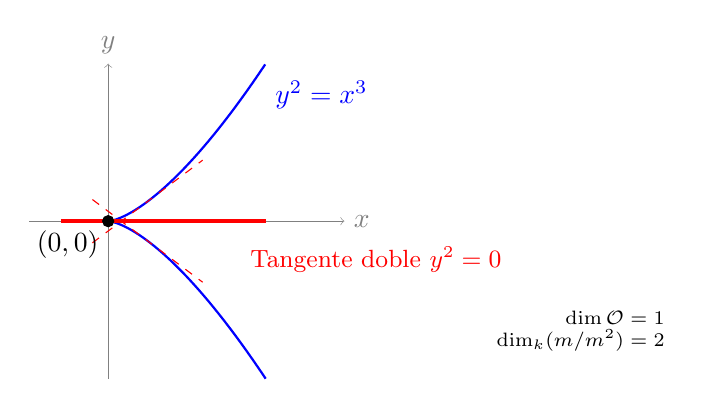
\begin{tikzpicture}[scale=2]
            % Ejes cartesianos
            \draw[->, help lines] (-0.5,0) -- (1.5,0) node[right] {$x$};
            \draw[->, help lines] (0,-1) -- (0,1) node[above] {$y$};
        
            % La cúbica cuspoidal y^2 = x^3 
            % Parametrización: x = t^2, y = t^3
            \draw[thick, blue, samples=100, domain=-1:1] plot ({\x*\x}, {\x*\x*\x});
            \node[blue, right] at (1,0.8) {$y^2=x^3$};
        
            % Rectas tangentes aproximándose (L1 y L2)
            % Tangente en t=0.5 (x=0.25, y=0.125) -> y - 0.125 = 0.75(x - 0.25)
            \draw[red, dashed, domain=-0.1:0.6] plot (\x, {0.75*\x - 0.0625});
            \draw[red, dashed, domain=-0.1:0.6] plot (\x, {-0.75*\x + 0.0625});
            
            % El límite: Espacio tangente doble (y=0)
            \draw[line width=1.5pt, red] (-0.3,0) -- (1,0);
            \node[red, below] at (1.7, -0.1) {\small Tangente doble $y^2=0$};
        
            % Punto singular en el origen
            \filldraw[black] (0,0) circle (1pt) node[anchor=north east] {$(0,0)$};
        
            % Notas aclaratorias
            \node[align=right, font=\scriptsize] at (3, -0.7) {
                $\dim \mathcal{O} = 1$ \\
                $\dim_k(\mathfrak{m}/\mathfrak{m}^2) = 2$ 
            };
        \end{tikzpicture}$$
    \end{ejem}
    ¿Es tangente en el origen?

    Consideramos la ecuación $x^3 + 0x^2 + 0x + y^2 = 0$. 
    ¿Cuál es su espacio tangente en el origen? 
    
    En este caso, la componente de menor grado (forma inicial) es $y^2 = 0$. Esto representa la recta $y=0$ contada 2 veces.
    
    Otro punto de vista: Graduados y Espacio Tangente
    
    Sea el morfismo de anillos dado por la proyección sobre $A$:
    $$\bt k{[x_i]} \rar{p \cdot} & k{[x_i]} \rar & A \rar & 0 \et$$
    Si consideramos el graduado asociado respecto al ideal maximal $\mathfrak{m}$, inducimos la sucesión:
    $$\bt G_{\m} k{[x_i]} \rar{p \cdot} & G_{\m} k{[x_i]} \rar & G_{\bar \m} A \rar & 0 \et$$
    
    Donde $G_{\mathfrak{m}} k[x_i] = k[x_i]$. Si $[p] \in \mathfrak{m}^r / \mathfrak{m}^{r+1}$, denotamos por $[p_r]$ su forma inicial de grado $r$. Luego, el graduado del anillo $A$ es:
    $$G_{\bar \m} A = \modulo{k{[x_i]}}{p \cdot k{[x_i]}} \simeq \text{Espacio Tangente}$$
    
    M\'as generalmente, si $A$ viene definido por varias ecuaciones $A = k[x_i]/(p_1, \dots, p_s)$, el espacio tangente es la intersección de los tangentes de cada $p_i = 0$. El conjunto de puntos $(\lambda_1, \dots, \lambda_n)$ del espacio tangente verifica:
    $$\{(\lambda_1, \dots, \lambda_n) \, / \, (p_1)_{r_1}(\lambda_1, \dots, \lambda_n) = 0, \dots, (p_s)_{r_s}(\lambda_1, \dots, \lambda_n) = 0\} $$
    Se prueba que el espacio tangente es, formalmente, $Spec(G_{\mathfrak{m}} A)$.
    \begin{defi}
        También se le llama \textbf{espacio tangente} al dual de $\modulo{\mathfrak{m}}{\mathfrak{m}^2}$. Es decir, $\left(\modulo{\mathfrak{m}}{\mathfrak{m}^2}\right)^*$ son los vectores tangentes.
    \end{defi} 

Sabemos que $\left(\modulo{\mathfrak{m}}{\mathfrak{m}^2}\right)^* = Der_k\left(A, \modulo{A}{\mathfrak{m}}\right)$, donde $\modulo{A}{\mathfrak{m}} \simeq k$. Dada una derivación $D$, $D: k[x_1, \dots, x_n] \longrightarrow k$ equivale a dar un elemento de $k^n$ (por la propiedad $Hom_{k-alg}$). Las derivaciones de $k[x_1, \dots, x_n]/(p_i)$ son aquellas derivaciones de $k[x_1, \dots, x_n]$ (elementos de $k^n$) que se anulan en el ideal generado por $p_i$.
\begin{ejem}
    $y^2 - x^3 = 0$

Una derivación $D$ es tangente si verifica:
$$\lambda \frac{\partial P}{\partial x}(0) + \mu \frac{\partial P}{\partial y}(0) = 0$$
En este caso, como las derivadas parciales en el origen son todas nulas ($0 + 0 = 0$), cualquier par $(\lambda, \mu)$ es una solución.

Si $(\lambda_1, \dots, \lambda_n) \in G_{\m} A$, entonces podemos definir la derivación como:
$$D = \sum \lambda_i \frac{\partial}{\partial x_i} \Big|_0$$
Lo cual constituye un vector tangente.

Formalmente, si consideramos el mapa $p: G_{\m} A \longrightarrow k$, donde $\lambda_i = p(x_i)$, esto nos permite identificar los puntos del esquema tangente con los vectores del espacio dual.
\end{ejem}
    
    